\documentclass[a4paper]{report}
\newcommand{\answerbox}[1][3\baselineskip]{
    \noindent\framebox[\linewidth]{
        \raisebox{0pt}[0pt][#1]{}
    }\par \medskip
}

%====================== PACKAGES ======================

\usepackage[english]{babel}
\usepackage[utf8x]{inputenc}
\usepackage{arabtex}
\usepackage{multirow}
\usepackage{utf8}
%pour gérer les positionnement d'images
\usepackage{float}
\usepackage{amsmath}
\usepackage{graphicx}
\usepackage{palatino}
\usepackage[final]{pdfpages}
\usepackage[colorinlistoftodos]{todonotes}
\usepackage{url}
\usepackage{amssymb}
\usepackage[resetfonts]{cmap}
\usepackage{fancyvrb}
\begin{VerbatimOut}{OT1.cmap}
%!PS-Adobe-3.0 Resource-CMap
%%DocumentNeededResources: ProcSet (CIDInit)
%%IncludeResource: ProcSet (CIDInit)
%%BeginResource: CMap (TeX-OT1-0)
%%Title: (TeX-OT1-0 TeX OT1 0)
%%Version: 1.000
%%EndComments
/CIDInit /ProcSet findresource begin
12 dict begin
begincmap
/CIDSystemInfo
<< /Registry (TeX)
/Ordering (OT1)
/Supplement 0
>> def
/CMapName /TeX-OT1-0 def
/CMapType 2 def
1 begincodespacerange
<00> <7F>
endcodespacerange
8 beginbfrange
<00> <01> <0000>
<09> <0A> <0000>
<23> <26> <0000>
<28> <3B> <0000>
<3F> <5B> <0000>
<5D> <5E> <0000>
<61> <7A> <0000>
<7B> <7C> <0000>
endbfrange
40 beginbfchar
<02> <0000>
<03> <0000>
<04> <0000>
<05> <0000>
<06> <0000>
<07> <0000>
<08> <0000>
<0B> <0000>
<0C> <0000>
<0D> <0000>
<0E> <0000>
<0F> <0000>
<10> <0000>
<11> <0000>
<12> <0000>
<13> <0000>
<14> <0000>
<15> <0000>
<16> <0000>
<17> <0000>
<18> <0000>
<19> <0000>
<1A> <0000>
<1B> <0000>
<1C> <0000>
<1D> <0000>
<1E> <0000>
<1F> <0000>
<21> <0000>
<22> <0000>
<27> <0000>
<3C> <0000>
<3D> <0000>
<3E> <0000>
<5C> <0000>
<5F> <0000>
<60> <0000>
<7D> <0000>
<7E> <0000>
<7F> <0000>
endbfchar
endcmap
CMapName currentdict /CMap defineresource pop
end
end
%%EndResource
%%EOF
\end{VerbatimOut}
%pour les informations sur un document compilé en PDF et les liens externes / internes
\usepackage[hypertexnames=false,bookmarks=true,bookmarksopen=true,colorlinks=true,citecolor=black,linkcolor=black, urlcolor= black, bookmarksdepth=3]{hyperref}
%pour la mise en page des tableaux
\usepackage{array}
\usepackage{tabularx}
\usepackage{mathtools}

%pour utiliser \floatbarrier
%\usepackage{placeins}
%\usepackage{floatrow}
%espacement entre les lignes
\usepackage{setspace}
%modifier la mise en page de l'abstract
\usepackage{abstract}
%police et mise en page (marges) du document
\usepackage[T1]{fontenc}
%Options: Sonny, 1Lenny, Glenn, 2Conny, 3Rejne, Bjarne, Bjornstrup
\usepackage[Lenny]{fncychap}
\usepackage[toc,page]{appendix}
\usepackage[top=2cm, bottom=2cm, left=2cm, right=2cm]{geometry}
%Pour les galerie d'images
\usepackage{subfig}

\usepackage{fancyhdr}

\setcode{utf8}
\pagestyle{fancy}
%====================== INFORMATION ET REGLES ======================

%rajouter les numérotation pour les \paragraphe et \subparagraphe
\setcounter{secnumdepth}{4}
\setcounter{tocdepth}{4}

\hypersetup{							% Information sur le document
pdfauthor = {Mèhdi Ben Hamida
		},			% Auteurs
pdftitle = {Big Data Management for Manufacturing Intelligence Application},			% Titre du document
pdfsubject = {Final Graduation Project Report},		% Sujet
pdfkeywords = {Big Data, Spark, HDFS, Data Analysis},	% Mots-clefs
pdfstartview={FitH},					% ajuste la page à la largueur de l'écran
pdfcreator = {MikTeX},% Logiciel qui a crée le document
pdfproducer = {National School of Computer Sciences}} % Société avec produit le logiciel
%title style declaration 

%======================== DEBUT DU DOCUMENT ========================

\begin{document}
\newcommand{\keyword}[1]{\textbf{#1}}
\newcommand{\tabhead}[1]{\textbf{#1}}
\newcommand{\code}[1]{\texttt{#1}}
\newcommand{\file}[1]{\texttt{\bfseries#1}}
 \newcommand{\option}[1]{\texttt{\itshape#1}}
\newcommand{\HRule}{\rule{\linewidth}{1mm}}

%page de garde
\begin{titlepage}
\fancypagestyle{test}{\fancyhf{}
\fancyhead[R]{June 2017}
\fancyhead[L]{Ref: 2017/II3/40}}
\thispagestyle{test}
\begin{center}

% Upper part of the page. The '~' is needed because only works if a paragraph has started.
\textsc{Ministry of Higher Education \\ for Scientific Research and Technology\\
University of Manouba\\National School of Computer Sciences}
\\[0.7cm]
   

\includegraphics[width=3.5cm,height=4cm]{./logoEnsi}~\\[1.5cm]

\textsc{\large Final Graduation Project Report}\\[1cm]

\textsc{ A Dissertation Submitted in Fulfillment of the Requirements for\\ \Large{\textbf{Computer Science Engineer Diploma}}}\\[0.5cm]

\HRule \\[0.4cm]
{\huge \bfseries Big Data Management for Manufacturing Intelligence Application \\[0.4cm] }
\HRule \\[0.5cm]

~\\
~\\

% Author and supervisor
\begin{minipage}{0.4\textwidth}
\begin{flushleft} \large
\emph{Performed By:}\\
\textbf{Mèhdi \textsc{\bf Ben Hamida}\\} 
\end{flushleft}
\end{minipage}
\begin{minipage}{0.4\textwidth}
\begin{flushright} \large
\emph{Supervised By:} \\
\textbf{Mr. Mohamed Anis \textsc{\bf Mlaouah}\\} 
\end{flushright}
\begin{flushright} \large
\emph{Academic Advisor:} \\
\textbf{Mrs. Lobna \textsc{\bf Jribi}\\} 
\end{flushright}
\end{minipage}


~\\
~\\
~\\
~\\

\textsc{\LARGE Hosting Company: }\\[0.3cm]

\includegraphics[width=7cm,height=2cm]{./iologo}~\\[0.4cm]
\textsc{Lake Gardens, Dollar Street Lake City Center Building Bloc A\\ 1st Floor, Tunis 1053 \\ Website: https://www.integrationobjects.com \\ Phone Number:+216 71 195 360}\\[1cm]


\vfill

% Bottom of the page
{\large Academic Year:}\\
{\large 2016-2017}

\end{center}
\end{titlepage}

%page blanche

~\\
~\\
~\\
~\\



\begin{center}
~\Large{Signature \& Stamp:} \\
\end{center}
~\Large{National School of Computer Sciences}\\
\answerbox[12\baselineskip]
~\Large{Integration Objects}\\
\answerbox[12\baselineskip]
%ne pas numéroter cette page
\thispagestyle{empty}
\newpage
\large
\renewcommand{\abstractnamefont}{\normalfont\Large\bfseries}
%\renewcommand{\abstracttextfont}{\normalfont\Huge}


\hskip7mm






\section*{Abstract}


\begin{spacing}{1.3}
In the world of Data Analysis, many features are proposed to perform data at a large scale in a fast, sure and intelligent process. Such a computing field is called BIG DATA. In this graduation project, we propose a Big Data Management for Manufacturing Intelligence Application. The main purpose of this project is to process statistics on a large set of data with features and functionalities performing knowledge extract from Big Data using appropriate tools.\\
\keyword{Keywords: Big Data, Spark, HDFS, Big Data Analytics}
\end{spacing}





\section*{Résumé}


\begin{spacing}{1.3}
Dans le monde de l'analyse des données, de nombreuses fonctionnalités sont proposées pour effectuer des données à grande échelle dans un processus rapide, sûr et intelligent. Un tel champ informatique s'appelle BIG DATA. Dans ce projet de fin d'études, nous proposons une application de gestion de Big Data pour la fabrication de l'intelligence. Le but principal de ce projet est d'exécuter des méthodes statistiques sur un large ensemble de données avec des fonctionnalités exécutant l'extrait de connaissances de Big Data en utilisant des outils appropriés.\\
\keyword{Mots clés: Données Enormes, Spark, HDFS, Analyse de Données}
\end{spacing}

\begin{flushright}
\section*{\<الملخص>}
\end{flushright}


\begin{spacing}{1.3}
\begin{arabtext}

في عالم تحليل البيانات، توجدالعديد من الميزات المقترحة لأداء البيانات على نطاق واسع في عمليات سريعة، مؤكدة وذكية. يسمى هذا المجال حوسبة البيانات الضخمة. في مشروع التخرج هذا، نقترح إدارة البيانات الكبيرة لتطبيق تصنيع الذكاء. والغرض الرئيسي من هذا المشروع هو معالجة الإحصاءات على مجموعة كبيرة من البيانات مع الميزات والوظائف لاستخراج المعرفة من البيانات الضخمة باستخدام الأدوات المناسبة.\\
\textbf{كلمات مفاتيح: البيانات الضخمة، سبارك، نظام هادوب للأنظمة الموزعة، تحليل البيانات}
\end{arabtext}
\end{spacing}




\vspace{\fill}
\thispagestyle{empty}
\newpage
\chapter*{}

\renewcommand{\abstractnamefont}{\normalfont\Large\bfseries}
%\renewcommand{\abstracttextfont}{\normalfont\Huge}


\hskip7cm

\vspace{\fill}
\begin{flushright}
\textit{"Software is a great combination between artistry and engineering."} \\[0.5cm]

\textbf{Bill Gates}
\end{flushright}

\vspace{\fill}




\thispagestyle{empty}
\newpage
%\chapter*{Glossaire}


\textbf{UML : } Unified Modeling Language \\

\textbf{RSFTA : } Service Réseau de Services Fixes de Télécommunications Aéronautiques \\

\textbf{BNI : } Bureau NOTAM International\\

\textbf{PIB : } Bulletins d’Information Pré-vol\\

\textbf{ADAMS : } Aeronautical Data And Message Handling System\\

\textbf{BIA : } Bureaux d’Information Aéronautique \\
\pagenumbering{roman}
%------- les entete
\renewcommand{\headrulewidth}{1pt}
\rhead{}
\lhead{\rightmark} 
\chead{} 
\renewcommand{\footrulewidth}{1pt}
\lfoot{\leftmark} 
\cfoot{}
\rfoot{\thepage}





\newpage
\chapter*{}



\hskip7mm



\begin{center}
\section*{Acknowledgement}

\end{center}

\begin{spacing}{1.3}
This dissertation was made possible through the patience and guidance of my advisor, \textbf{Mrs. Lobna Jribi}. I am most grateful for her constant support and encouragements that brought my work in the right direction.\\

I would like to thank also my beloved family for their continuous encouragement, support and help in every step that I make. You provide me the strength that I need to go forward.\\

I would also like to thank the members of the jury for taking the time to evaluate my work and give me valuable feedback.\\

Kind regards go to my internship supervisors and collaborators: \textbf{Mr. Mohamed Anis Mlaouah}, \textbf{Mr. Mohamed Mehdi Sidommou} and \textbf{Mrs. Imen Majed}. I am grateful for giving me the chance to work with you and for all your mentoring advices. You have all helped me to improve my work and myself.\\

I would also like to thank a number of friends that were particularly supportive along this path. All my gratitude to my \textbf{National School of Computer Sciences} classmates. Many thanks to my \textbf{Preparatory Institute for Engineering Studies-El Manar} classmates with whom I closely shared many enlightening experiences during two years of preparatory studies.\\

Finally, many thanks to all other people that had a direct or indirect contribution to this work and were not explicitly mentioned above. Your help and support is very much appreciated.\\
\end{spacing}

\chapter*{Abbreviations}



\begin{table}[H]

\begin{center}

\begin{tabularx}{17cm}{ p{1.8cm}X } 
\textbf{\large{HDFS:}}  & \large{Hadoop Distributed File System} \newline \\
\textbf{\large{IO:}}   & \large{Input/Output} \newline\\
\textbf{\large{ML}}   & \large{Machine Learning} \newline \\
\textbf{\large{MLlib}} & \large{Machine Learning Library} \newline \\
\textbf{\large{PCA:}}  & \large{Principal Component Analysis}\newline \\
\textbf{\large{RDD:}}   &  \large{Resilient Distributed Dataset}\newline \\
\textbf{\large{RPC:}}   &  \large{Remote Procedure Call}\newline \\
\end{tabularx}
\end{center}
\end{table}
\tableofcontents
\listoffigures
\listoftables
\large
%ne pas numéroter le sommaire



%espacement entre les lignes d'un tableau
\renewcommand{\arraystretch}{1.5}

%====================== INCLUSION DES PARTIES ======================


\newpage
\thispagestyle{empty}
%recommencer la numérotation des pages à "1"
\pagenumbering{arabic}
\setcounter{page}{1}
\newpage
\newpage
\newpage
\thispagestyle{empty}
\renewcommand{\labelitemi}{$\bullet$}
\renewcommand{\labelitemii}{$\circ$}
%------- les entete
\renewcommand{\headrulewidth}{1pt}
\rhead{}
\lhead{\rightmark} 
\chead{} 
\renewcommand{\footrulewidth}{1pt}
\lfoot{\leftmark} 
\cfoot{}
\rfoot{\thepage}
%including the chapters 
\chapter*{Introduction générale} % Pas de numérotation
\addcontentsline{toc}{chapter}{Introduction générale}


Depuis l’invention du premier avion en 1903 appelé Wright Flyer, la gestion de trafic aérien fut un des défis les plus difficiles à résoudre vu le nombre des vols ascendants. Cette gestion a pour but de maintenir en sécurité le trafic aérien, d’ou l’apparition des organismes internationaux qui s’occupent de cette tâche. L’OACI, Office d’Aviation Civile International est l’organisme qui se charge d’établir les protocoles standardisés de de communication entre les différents aérodromes partout dans le monde. Il normalise aussi les types de messages échangés ainsi que les canaux de transfert utilisés. L’OACA, Office des Aéroport et d’Aviation Civile, qui dérive de l’OACI, est l’organisme nationale qui s’occupe de l’espace aérien tunisien. Sa tâche est de s'occuper de tout ce qui est en relation avec les aéroports internationaux existants sur le territoire tunisien. Cet organisme est décomposé en plusieurs divisions, parmi lesquelles on cite; le centre de contrôle régional. \\

Dans le domaine du contrôle aérien, un centre de contrôle régional, est un centre assurant la sécurité du trafic aérien. L’échange de messages aéronautiques entre ces centres assure l’exécution sûre, rapide et efficace des vols. Il consiste aussi à accélérer et ordonner la circulation aérienne. C’est pour cela que la disponibilité des liaisons entre ces centres s’avère indispensable décisif vu son importance dans la sécurité de la navigation aérienne, la régularité des vols, et le traitement des messages aéronautiques. \\

La diponibilité des messages aéronautiques est un affaire indispensable. Dans ce cadre, s'inscrit notre projet de stage d'immersion en entreprise qui a pour but la conception et la réalisation d'une solution d'apurement de la base de données du système STANOS.\\

Le présent rapport s'organise autour de cinq chapitres:\\
Le premier chapitre intitulé {\bf "Présentation générale"} comprend une présentation de l'organisme dans lequel nous avons effectué notre stage. Il comprend aussi une définition du système autour duquel se déroule notre stage. \\
Le deuxième chapitre intitulé {\bf "Étude préalable"} comprend une revue théorique des notions sur lesquelles s’appuie notre projet en une étude de l’existant, des critiques et une proposition solution à notre problématique.\\
Le troisième chapitre intitulé  {\bf "Analyse et spécification des besoins"} expose la spécification des besoins fonctionnels et non fonctionnels de l’application.\\
Un quatrième chapitre intitulé  {\bf "Conception"} met en évidence la modélisation conceptuelle de l’application.\\
Le dernier chapitre intitulé  {\bf "Réalisation"} inclut une présentation de l’environnement de travail avec la description de quelques interfaces de l’application.\\

Enfin, nous clôturons ce rapport par une conclusion générale dans laquelle nous résumons notre solution et exposons quelques perspectives futures.\\
\chapter{Project Overview} 
\label{Chapter1} 
Throughout this first chapter, we will present the hosting organism. We will, also, present the frame of our project, introduce its framework and define its goal. Then, we will take care to present the problem statement as well as the purpose of this project.
\section{Hosting Organism}
\subsection{Overview}
\textbf{Integration Objects} is a software development company, created in 2002, based in Tunisia with sales representatives in Texas and Genoa. Over the last decade, it has built and maintained a strong reputation as a leading systems integrator and solutions provider for knowledge management, automation, plant process management and decision support applications. It is specialized in delivering solutions that monitor plant, supply chain operation performance, and identify opportunities to increase profitability.\\

\textbf{Integration Objects} offers highly scalable and reliable solutions that allow real-time data collection from multiple plant systems and various enterprise networks. This enables companies to turn data, information, and knowledge into operational intelligence, thereby optimizing their business and manufacturing processes.\\

\textbf{Integration Objects} provides two main categories of software products:
\begin{itemize}
\item \textbf{Operational Intelligence:} The core objectives of this product category are to empower customers' operations, to increase production up-time and to maximize asset availability, normal operations and safety. The product suite includes applications for performance
monitoring using key performance indicators, plant operations management, abnormal condition management, predictive analytics, asset management and decision support. These applications are built on top of Integration Objects' platform, KnowledgeNet Analytics
and Smart Equipment.
\item \textbf{Standard Industry Connectivity \& Cyber Security:} This product category includes more than 40 OPC based software products enabling users to integrate their systems using industry communication standards. These products enable enterprise systems and devices to access process data, alarm and event messages and historical data. This data is collected from devices such as sensors or Programmable Logic Controller (PLC).\\
\end{itemize}

Thanks to the quality and management standards, Integration Objects is a certified \textbf{ISO 9001:2008}. It is also an active member of:
\begin{itemize}
\item \textbf{OPC Foundation:} OPC Foundation is a global organization in which users, vendors and consortia collaborate to create data transfer standards for multi-vendor, multi-platform, secure and reliable interoperability in industrial automation.
\item \textbf{The International Society of Automation (ISA):} Founded in 1945, the International Society of Automation is a leading, global, non-profit organization with more than 40,000 members worldwide. ISA develops standards, certifies industry professionals, provides education and training, publishes books and technical articles, and hosts conferences and exhibitions for automation professionals.
\item \textbf{Machinery Information Management Open System Alliance (MIMOSA):} MIMOSA is a not-for-profit trade association dedicated to developing and encouraging the adoption of open information standards for Operations and Maintenance in manufacturing, fleet, and facility environments.\\
\end{itemize}

By such memberships, it aims to provide services and products that enable interoperability between different applications and different suppliers. They are aligned with the highest industry standards.

\subsection{Work Methodology}
To enhance product quality and accelerate the process of software development, Integration Objects implemented a methodology helping engineers in the design and development of software. This methodology is based on the ISO 9001 process approach 2008 version.\\

During our internship, this methodology was adopted. It requires a validation phase in
between main stages whenever necessary. It also, recommends the use of prototypes throughout the iterative project’s life cycle (see figure \ref{fig2}). In each stage we create specific documents that sum up the work done in the stage and serve as a starting point for the following one.
\begin{figure}[!ht]
\begin{center}
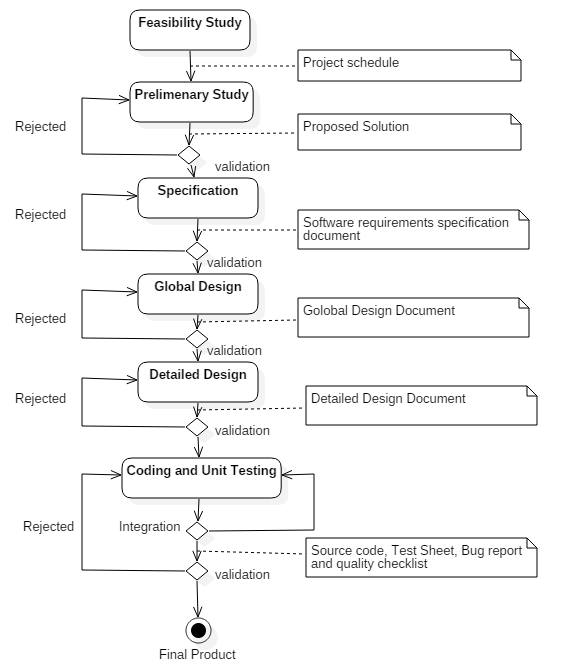
\includegraphics[width=14.8cm,height=17.8cm]{chapter1/fig2.png}
\end{center}
%légende de l'image
\caption{Integration Objects Work Methodology}
\label{fig2}
\end{figure}
\begin{itemize}
\item \textbf{Feasibility Study:} It is the first stage of the ISO process through which determines and to documents the project’s viability. \\ \textbf{Stage Output:} Project Schedule.
\item \textbf{Preliminary Study:} It represents an initial exploration of existing and possible solutions to the issue addressed. \\ \textbf{Stage Output:} Proposed solution.
\item \textbf{Specification:} This stage describes the client’s needs and determines the system features.\\ \textbf{Stage Output:} Software requirements specification document.
\item \textbf{Global Design:} The fourth stage describes the architecture of the product and its main parts. \\ \textbf{Stage Output:} Global design document.
\item \textbf{Detailed Design:} In this stage, we determine how to efficiently structure the main parts defined in the previous stage. \\\textbf{Stage Output:} Detailed design document.
\item \textbf{Coding and unit testing:} Developers have to implement the entire solution according to the design and to validate functional features. \\\textbf{Stage Output:} Source code, Test sheet, Bug report and quality checklist.
\end{itemize}
\section{Project Description}
\subsection{Scope}

This document is the \textbf{Graduation Project Dissertation} for a design and implementation of a \textbf{Big Data Management for Manufacturing Intelligence Application}. Throughout this document we will define the project's context and present it. This document will describe the methodology followed while realizing this project.


This project is a requirement for the final year in the \textbf{National School of Computer Science} in order to obtain the National Diploma of a Computer Sciences Engineer. It has been achieved during an internship
at \textbf{Integration Objects} that lasted 4 months starting from February $1^{st}$, 2017 to May $31^{th}$, 2017.

\subsection{Project Description}

\textbf{KnowledgeNet Analytics} is an out of the box data analysis software product, designed to meet operations needs in terms of knowledge mining in order to unlock hidden knowledge and profits within plant historical data. \textbf{KnowledgeNet Analytics} helps analyzing and investigating the plant process behavior and states, identifying opportunities to increase operational efficiency and reliability, and predicting abnormal conditions. One of the known issues in this field is how to manage huge volumes of data in term of storage, algorithms optimizations and presentation. The purpose of this project is to study and provide the best way for big data management.\\

The main objective of this project is to:
\begin{itemize}
\item Perform a literature review to understand the project scope
\item Engineer the best technical solution to load and manage huge volumes of data into a new built platform
\item Apply standard operations such as matrix operations and complex algorithms (PCA (Principal Components Analysis) and Linear Regression, etc.) using the best solution for big data
\item Compare results with other products
\end{itemize}
\section*{Conclusion}
This chapter was meant to set the general context in which our project took place. We presented the hosting company, isolated our project's goals and briefly described it. In the next chapter, we will establish a theoretical study, and we will be dealing with basic concepts relevant to our project while evaluating existing solutions. 
\chapter{Preliminary Study} 
\label{Chapter2}
In this chapter, we will proceed through two sections; the first one will define a theoretical background which will be used in this project to solve its problematic. The second one will cover a study of the existing technologies and establish a comparative analysis in order to pick a technical review as a result.
\section{State of the Art}
\subsection{Concepts of Big Data}
\subsubsection{Definitions}
Big Data is a data whose scale, diversity, and complexity require new architecture, techniques, algorithms, and analytics to manage it and extract value and hidden knowledge from it. Traditional databases analytics says what happened and what is happening, however gives the predictive analysis of what is likely to happen in future. Infrastructure requirements of big data are data acquisition, data organization and data analysis \cite{cite16}. \\

The term "Big Data" describes innovative techniques and technologies to capture, store, distribute, manage and analyze
petabyte- or larger-sized datasets with high-velocity and different structures. Big data can be structured, unstructured or semi-structured, resulting in incapability of conventional data management methods \cite{cite17}.\\

Big Data refers to the explosion in the quantity and sometimes quality of available and potentially relevant data, largely the result of recent and unprecedented advancements in data recording and storage technology. In this new and exciting world, sample sizes are no longer measured in number of observations, but rather in megabytes.\\

The most popular definition in the recent years is the "Three V's": volume, velocity , and variety. The concept was first raised by Doug Laney (2001) in his META Group
research note \cite{cite} that describes the characteristics of datasets that cannot be handled by traditional data management tools. With the development of discussion and increasing interest in big data, the "Three V's" have been expanded to "Five V’s": volume, velocity, variety, veracity, value and now it's about multi-V model.
\subsubsection{The 3-V Model}
\label{3vm}
It is generally accepted that big data can be explained according to three V's: Velocity, Variety and Volume.\\

\begin{itemize}
\item \textbf{Velocity:} The phrase velocity represents the data generation speed. Big data velocity deals with the step at which data flows in from sources like business processes, machines, networks and human interaction with things like social media sites, mobile devices etc. The flow of data is massive and continuous. This real time data can help users make valuable decisions. Thus, velocity means analyzing of streaming data.\\

\item \textbf{Variety:} Variety refers to the many sources and types of data, both structured and unstructured. The data is stored in spreadsheets and databases, which comes from different sources. Now data comes in the form of csv files, photos, videos, monitoring devices, PDF, Audio etc. This variety of unstructured data creates problems for storage, mining and analyzing data. In order to defeat this issue, we have to define the data storage system which can analyze variety of data.\\

\item \textbf{Volume:} Big Data implies enormous volumes of data. This data is generated and created for different purposes by machines, networks and human interaction on systems. The volume of data to be analyzed is a huge amount of data. Recently, the data generation sources are augmented and it causes diversity of data such as text, video, audio and databases. In order to process the enormous amount of data, conventional data processing has to be enhanced.\\
\end{itemize}


\subsubsection{From 3-V to multi-V Model}

Big data initially meant the volume, velocity and variety of data that becomes
tricky to analyze by using conventional data processing platforms and techniques. Nowadays, data production sources are improved rapidly, such as sensor networks, high throughput instruments, streaming machines and these environments generate massive amount of data.\\

Nowadays, big data has been playing a crucial role in a variety of environments such as business organization, industry, scientific research, natural resource management, social networking and public administration, and the 3'Vs model is no longer suitable to print the big data features. Therefore, a multi-V model is adopted \cite{cite18}.\\


\begin{itemize}
\item \textbf{Velocity,Variety and Volume:} already defined in section \ref{3vm}.  
\item \textbf{Value:} The value of data indeed represents Big Data. Having continuous amounts of data is not helpful until it can be turned into value. It is essential to understand that doesn't always mean there is value in Big Data. The benefits and costs of analyzing and collecting the big data is more impartment thing when doing big data analytics.
\item \textbf{Veracity:} Veracity represents the data understandability; it
doesn't represent data quality. It is significant that the association should perform data processing to prevent "dirty data" from accumulating in the systems. 
\item \textbf{Validity:} It
is essential to ensure whether the data is precise and accurate for the future use. In
order to take the right decisions in future, the organizations should valid the data
noticeably.
\item \textbf{Variability:} Variability refers to the data consistent and data value.
\item \textbf{Viscosity:} Viscosity is an element of velocity and it represents the latency or lag time in data transmit between the source and destination. 
\item \textbf{Virality:} Virality represents the speed of the data send and receives from various sources.
\item \textbf{Visualization:} Visualization is used symbolize the Big Data in a complete view and determine the hidden values. Visualization is an essential key to making big data an integral part of decision making.
\end{itemize}
\subsubsection{Big Data Analysis}
Techniques for efficiently accessing, analyzing and presenting large amounts of
dynamic, heterogeneous data, with the goal of obtaining new knowledge and facts, play
an increasingly important role in various application domains, such as media, patent
databases, scientific repositories, medical databases etc.\\

Since data is not always moved during the organization step, the analysis may also be done in a distributed environment, where some data will stay where it was
originally stored and be transparently accessed from a data warehouse. The infrastructure required for analyzing big
data must be able to support complex analytics such as statistical analysis and data mining, on a wider variety of
data types stored in diverse systems, scale to extreme data volumes, deliver faster response times driven by changes in
behavior and automate decisions based on analytical models.\\

Most importantly, the infrastructure must be able to integrate analysis on the combination of big data and traditional enterprise data. New insight comes not just from analyzing new data, but from analyzing it within the context of the old to provide new perspectives on old problems. Figure \ref{process} shows the data analysis process.\\

~\\

\begin{figure}[!ht]
\begin{center}
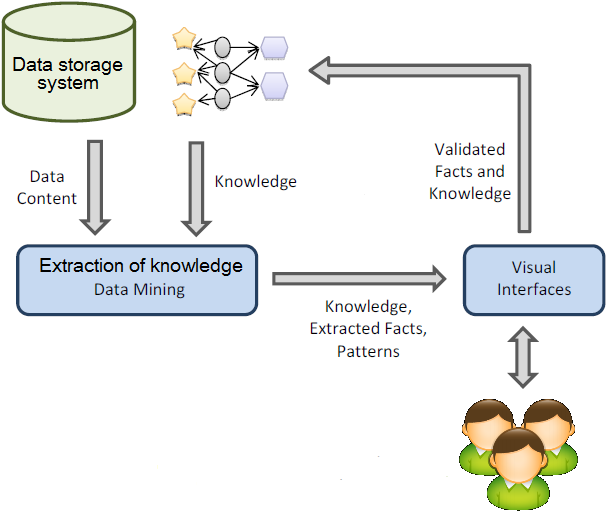
\includegraphics[width=15cm,height=9.8cm]{chapter2/fig9.png}
\end{center}
%légende de l'image
\caption{Data Analysis Process}
\label{process}
\end{figure}
~\\
\subsubsection{Required Infrastructure for Big Data}

Even though the data will be in distributed environment, infrastructure must support to carry out very high transaction volumes and also support flexible data structures. To collect and store data, csv files are often used in big data. Csv files (Comma Separated Values) will not have any fixed schema since it supports high variety of data by capturing all types of data.\\

In the classical term of data warehousing, organizing data is called as data integration. Big data requires good infrastructure, so that processing and manipulating data in the original storage location can be done easily. It must also supports very high throughput to deal with processing steps of large data and handles large variety of data formats like structured format, unstructured format and others. Hadoop is a new technology that allows large data volumes to be organized and processed while keeping the data on the original data storage cluster. Many others distributed frameworks, working over hadoop, are available for data processing. The purpose of this frameworks is to facilitate analytics and improve performance. 

\subsection{Data Mining Tools}
The recent increase of dataset size, in number of records as well as of attributes, has triggered the development of a number of big data platforms as well as parallel data analytics algorithms. At the same time though, it has pushed for the usage of many techniques to extract knowledge from a large set of data. In this section, we will define the main tools used for knowledge extract from data. We have chosen three types of tools which are: dimensionality reduction, clustering and supervised learning algorithms.
\subsubsection{Dimensionality Reduction Procedures}
\label{sectionpca}
Before proceeding with any data analytics task, we need to implement one or more dimensionality reduction techniques. Dimensionality reduction is not only useful to speed up algorithm execution, but actually might help with the final classification or clustering accuracy as well \cite{cite10}.\\ 

\textbf{\normalsize{Principal Component Analysis}}\\

Principal Component Analysis (PCA) is the general name for a technique that uses sophisticated underlying mathematical principles to transforms a number of possibly correlated variables into a smaller number of variables called principal components. The origins of PCA lie in multivariate data analysis, however, it has a wide range of other applications. PCA is one of the most results from applied linear algebra \cite{cite9} and its most common use is to analyse large dataset. It can also be used in de-noising signals, blind source separation and data compression.\\

In general terms, PCA uses a vector space transform to reduce the dimensionality of large data sets. Using mathematical projection, the original data set, which may have involved many variable, can often be interpreted in just a few variables (the principal components). The aim of this section is to explain the theoretical side of PCA.\\

\textbf{\normalsize{The Technical Details of PCA}}\\

As we have mentioned previously, the Principal Component Analysis is above to take a large set of data and identify an optimal new basis in which to re-express the data. \\

The general aim of the PCA method is to find another basis that is a linear combination of the original basis and that re-expresses the data optimally. Let us frame the problem in the following way:\\

Assume that we start with a data set that is represented in terms of an $m \times n$ matrix, $X$ where the $n$ columns are the samples (e.g. observations) and the m rows are the variables. We want to linearly transform this matrix, $X$ into another matrix, $Y$, also of dimension $m \times n$, so that for some $m \times m$ matrix, $P$.\\ 
~\\
\begin{equation*}
\label{eq1}
PX = (Px_{1} Px_{2} \ldots Px_{n})
=
\begin{pmatrix}
    p_{1}x_{1} & p_{1}x_{2}  & \dots  & p_{1}x_{n} \\
    p_{2}x_{1} & p_{2}x_{2}  & \dots  & p_{2}x_{n} \\
    \vdots & \vdots  & \ddots & \vdots \\
    p_{m}x_{1} & p_{m}x_{2}  & \dots  & p_{m}x_{n}
\end{pmatrix}
=
Y
\end{equation*}
~\\ ~\\ 
This equation represents a change of basis. Note that $p_{i},x_{j} \in  \mathbb{R}^{m}$. This tell us that the original data, $X$ is being projected on the column of $P$. Thus, the rows of $P$, $\{ p_{1},p_{2},\ldots,p_{m} \}$ are a new basis for representing the columns of $X$. The rows of P will later become the principal components directions.\\

More details about the principal component analysis in appendix \ref{appendixpca}.


\subsubsection{Clustering}
Clustering is a procedure that divides data into groups which are meaningful, useful, or both. In order to get meaningful group, clusters should capture the natural structure of the data. In some cases, cluster analysis is a useful starting for other purposes, such as data summarization. Other to data analysis, clustering plays an important role in a wide variety of fields: psychology, social sciences, biology and data mining. There have been many applications of cluster analysis to practical problems. \\

Before discussing specific clustering techniques, we provide some necessary background. First, we further define cluster analysis, illustrating why it's difficult. Then, we will explore different techniques that group data.\\

\textbf{\normalsize{Cluster Analysis}}\\

Cluster analysis groups data objects based only on information found in the data that describes the objects and their relationships. The goal is that the objects within a group be similar to one another and different from the objects from the other groups \cite{cite11}. The greater the similarity within a group and the greater the difference between groups, the more distinct the clustering. Figure \ref{fig4} shows three different ways to divide a set of points into clusters. \\
\begin{figure}[H]
\begin{center}
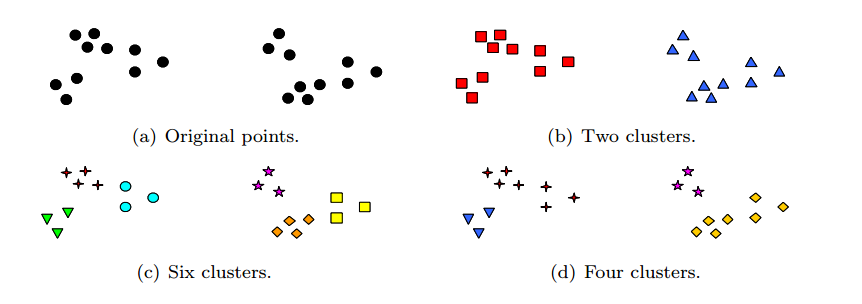
\includegraphics[width=15cm,height=7cm]{chapter2prime/fig1.png}
\end{center}
%légende de l'image
\caption{Different Ways of Clustering the same Set of Points}
\label{fig4}
\end{figure}

\textbf{\normalsize{Approaches to cluster analysis}}\\

There are a number of different methods that can be used to carry out a cluster analysis;
these methods can be classified as follows:
\begin{itemize}
\item Hierarchical methods:
\begin{itemize}
\item Agglomerative methods, in which subjects start in their own separate cluster. The
two "closest" (most similar) clusters are then combined and this is done repeatedly
until all subjects are in one cluster. At the end, the optimum number of clusters is
then chosen out of all cluster solutions.
\item Divisive methods, in which all subjects start in the same cluster and the above strategy is applied in reverse until every subject is in a separate cluster. Agglomerative methods are used more often than divisive methods, so this handout will
concentrate on the former rather than the latter.
\end{itemize}
\item Non-hierarchical methods (often known as k-means clustering methods)
\end{itemize}

\textbf{\normalsize{Data and Measures of Distance}}\\

The data used in cluster analysis can be interval, ordinal or categorical. However, having a mixture of different types of variable will make the analysis more complicated. This is because in cluster analysis we need to have some way of measuring the distance between observations
and the type of measure used will depend on what type of data we have.\\

A number of different measures have been proposed to measure distance for binary and categorical data. For interval data the most common distance measure used is the Euclidean distance. In general, if we have $p$ variables $X_{1},X_{2},\ldots,X_{p},$ measured on a sample of n subjects, the observed data for subject $i$ can be denoted by $x_{i1},x_{i2},\ldots,x_{ip}$ and the observed data for subject $j$ by $x_{j1},x_{j2},\ldots,x_{jp}$. The Euclidean distance between these two subjects in given by:\\
\begin{equation*}
d_{ij}=\sqrt{(x_{i1}-x_{j1})^{2}+(x_{i2}-x_{j2})^{2}+\ldots+(x_{ip}-x_{jp})^{2}}
\end{equation*} 
~\\ ~\\
\textbf{\normalsize{Hierarchical Agglomerative Methods}}\\

Within this approach to cluster analysis there are a number of different methods used to determine which clusters should be joined at each stage \cite{cite19}. The main methods are summarised below \cite{cite20}: 
\begin{itemize}
\item \textbf{Nearest neighbour method (single linkage method):} In this method the distance between two clusters is defined to be the distance between the two closest members, or neighbours. This method is relatively simple but is often criticised because it doesn't take account of cluster structure and can result in a problem called chaining whereby clusters end up being long and straggly. However, it is better than the other methods when the natural clusters are not spherical or elliptical in shape.
 
\item \textbf{Furthest neighbour method (complete linkage method):} In this case the distance between two clusters is defined to be the maximum distance between members — i.e. the distance between the two subjects that are furthest apart. This method tends to produce compact clusters of similar size but, as for the nearest neighbour method, does not take account of cluster structure. It is also quite sensitive to outliers.

\item \textbf{Average (between groups):} linkage method (sometimes referred to as UPGMA) The distance between two clusters is calculated as the average distance between all pairs of subjects in the two clusters. This is considered to be a fairly robust method.

\item \textbf{Centroid method:} Here the centroid (mean value for each variable) of each cluster is calculated and the
distance between centroids is used. Clusters whose centroids are closest together are merged. This method is also fairly robust.

\item \textbf{Ward's method:} In this method all possible pairs of clusters are combined and the sum of the squared
distances within each cluster is calculated. This is then summed over all clusters. The combination that gives the lowest sum of squares is chosen. This method tends to produce clusters of approximately equal size, which is not always desirable. It is also quite sensitive to outliers. Despite this, it is one of the most popular methods, along with the average linkage method.

\end{itemize}

It is generally a good idea to try two or three of the above methods. If the methods agree reasonably well then the results will be that much more believable.\\

\textbf{\normalsize{K-means Clustering}}\\

k-means clustering is a method of vector quantization, that is popular for cluster analysis in data mining. k-means clustering aims to partition n observations into k clusters in which each observation belongs to the cluster with the nearest mean, serving as a prototype of the cluster. This results in a partitioning of the data space into Voronoi cells.
K-means clustering is a method commonly used to automatically partition a data set into k groups. It proceeds by selecting k initial cluster centers and then iteratively refining them as follows:
\begin{itemize}
\item Each instance $d_i$ is assigned to its closest cluster center.
\item Each cluster center $C_j$ is updated to be the mean of its constituent instances.
\end{itemize}

The algorithm converges when there is no further change in assignment of instances to clusters.
\newpage
\subsubsection{Supervised Learning}
Supervised Learning is simply a formalization of the idea of learning from examples. In supervised learning, the learner is provided with two sets of data, a training set and a test set. The idea is for the learner to learn from a set of labeled examples in the training set so that it can identify unlabeled exemples in the test set with the highest possible accuracy \cite{cite21}.\\

A supervised learning algorithm analyzes the training data and produces an inferred function, which is called a classifier, if the output is discrete, or a regression function, if the output is continuous. \\

\textbf{\normalsize{Linear Regression}}\\

Linear regression is an approach for modelling the relationship between a scalar dependent variable y and one or more explanatory (independent) variables. It is used for correlation analysis and tries to come up with the best model that fits the values of independent variables. \\

Linear regression is used for predicting the value of dependent variable with as little error as possible rather than predicting the class label. In order to do this, it needs to learn the correlated features by calculating the linear coefficients of the independent variables according to the following formula:\\ 

\begin{equation*}
y_{i}=\beta_{1}x_{i1}+\ldots+\beta_{p}x_{ip}+\varepsilon_{i}=X_{i}^{T}\beta+\varepsilon_{i}, i=1,\ldots,n
\end{equation*}

As seen from the regression formula, a linear regression model assumes that the relationship between the dependent variable $y_{i}$ and the vector of regressors $x_i$ is linear. Error variable $\varepsilon_{i}$ is an unobserved random variable that adds noise to the linear relationship between the dependent variable and regressors.\\

After coefficients are calculated through learning and model is created that will produce the red line in figure \ref{Regression}, this model will be used to predict the value of the dependent variable based on the input values of the independent variables.\\
\begin{figure}[H]
\begin{center}
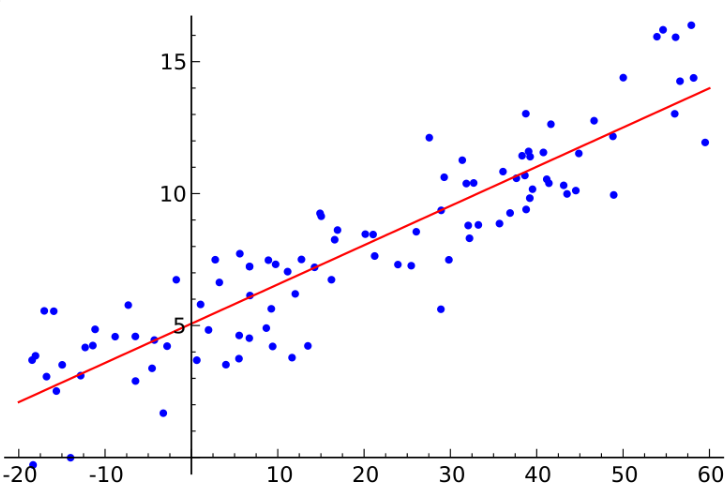
\includegraphics[width=14.5cm,height=7.5cm]{chapter2prime/lr.png}
\end{center}
%légende de l'image
\caption{Linear Regression Representation}
\label{Regression}
\end{figure}


\textbf{Evaluation Metrics for Model Correctness:} Calculation of residuals is crucial for assessing the correctness of the regression model. Residuals are the differences between the observed and predicted values by the model. Using these residual values, evaluation metrics can be calculated:\\

The sum of squared residuals (SSE):
\begin{align*}
SSE&=\Sigma(y_{i}-\widehat{y_{i}})^2\\
R^{2}_{a}&=\dfrac{[(n-1)R^{2}-k]}{[n-(k+1)]}\\
\hat{\sigma}^2 &=\dfrac{SSE}{n-(k+1)}=MSE
\end{align*}

The sum of squared total residuals (SST):
\begin{align*}
SST&=\Sigma(y_{i}-\bar{y}_{0})^{2} \\
f&=\dfrac{R^2/k}{(1-R^{2})/[n-(k+1)]} \\R^2 &= 1-\dfrac{SSE}{SST}
\end{align*}


\textbf{\normalsize{Classifications}}\\

Classification is an instance of supervised learning \cite{cite22}. It is the problem of identifying to which of a set of categories a new observation belongs, on the basis of a training set of data containing observations  whose category membership is known. Classification is an example of pattern recognition. Classification is an example of the more general problem of pattern recognition, which is the assignment of some sort of output value to a given input value. Figure \ref{classification} shows the classification process.\\
~\\ ~\\
\begin{figure}[H]
\begin{center}
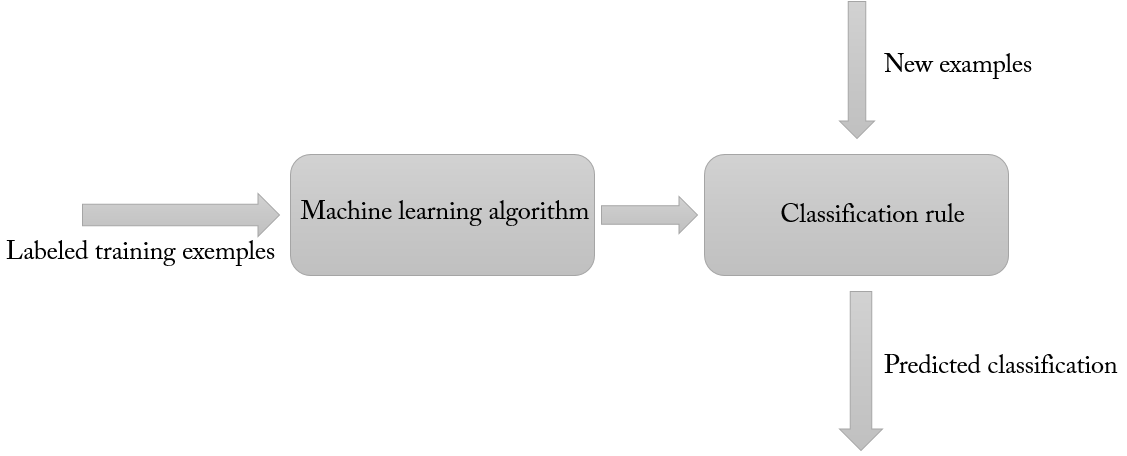
\includegraphics[width=16.5cm,height=7.5cm]{chapter2prime/fig3.png}
\end{center}
%légende de l'image
\caption{Classification Process}
\label{classification}
\end{figure}
\newpage
Example of classification algorithms include:
\begin{itemize}
\item Linear classifiers
\begin{itemize}
\item Fisher's linear discriminant
\item Logistic regression
\item Naive Bayes classifier
\item Perceptron
\end{itemize}
\item Support vector machines
\item Quadratic classifiers
\item Kernel estimation
\begin{itemize}
\item k-nearest neighbor
\end{itemize}
\item Decision trees
\begin{itemize}
\item Random forests 
\end{itemize}
\item Neural networks
\item Learning vector quantization
\end{itemize}

A review of data analysis techniques is represented in figure \ref{analysis}.
\begin{figure}[H]
\begin{center}
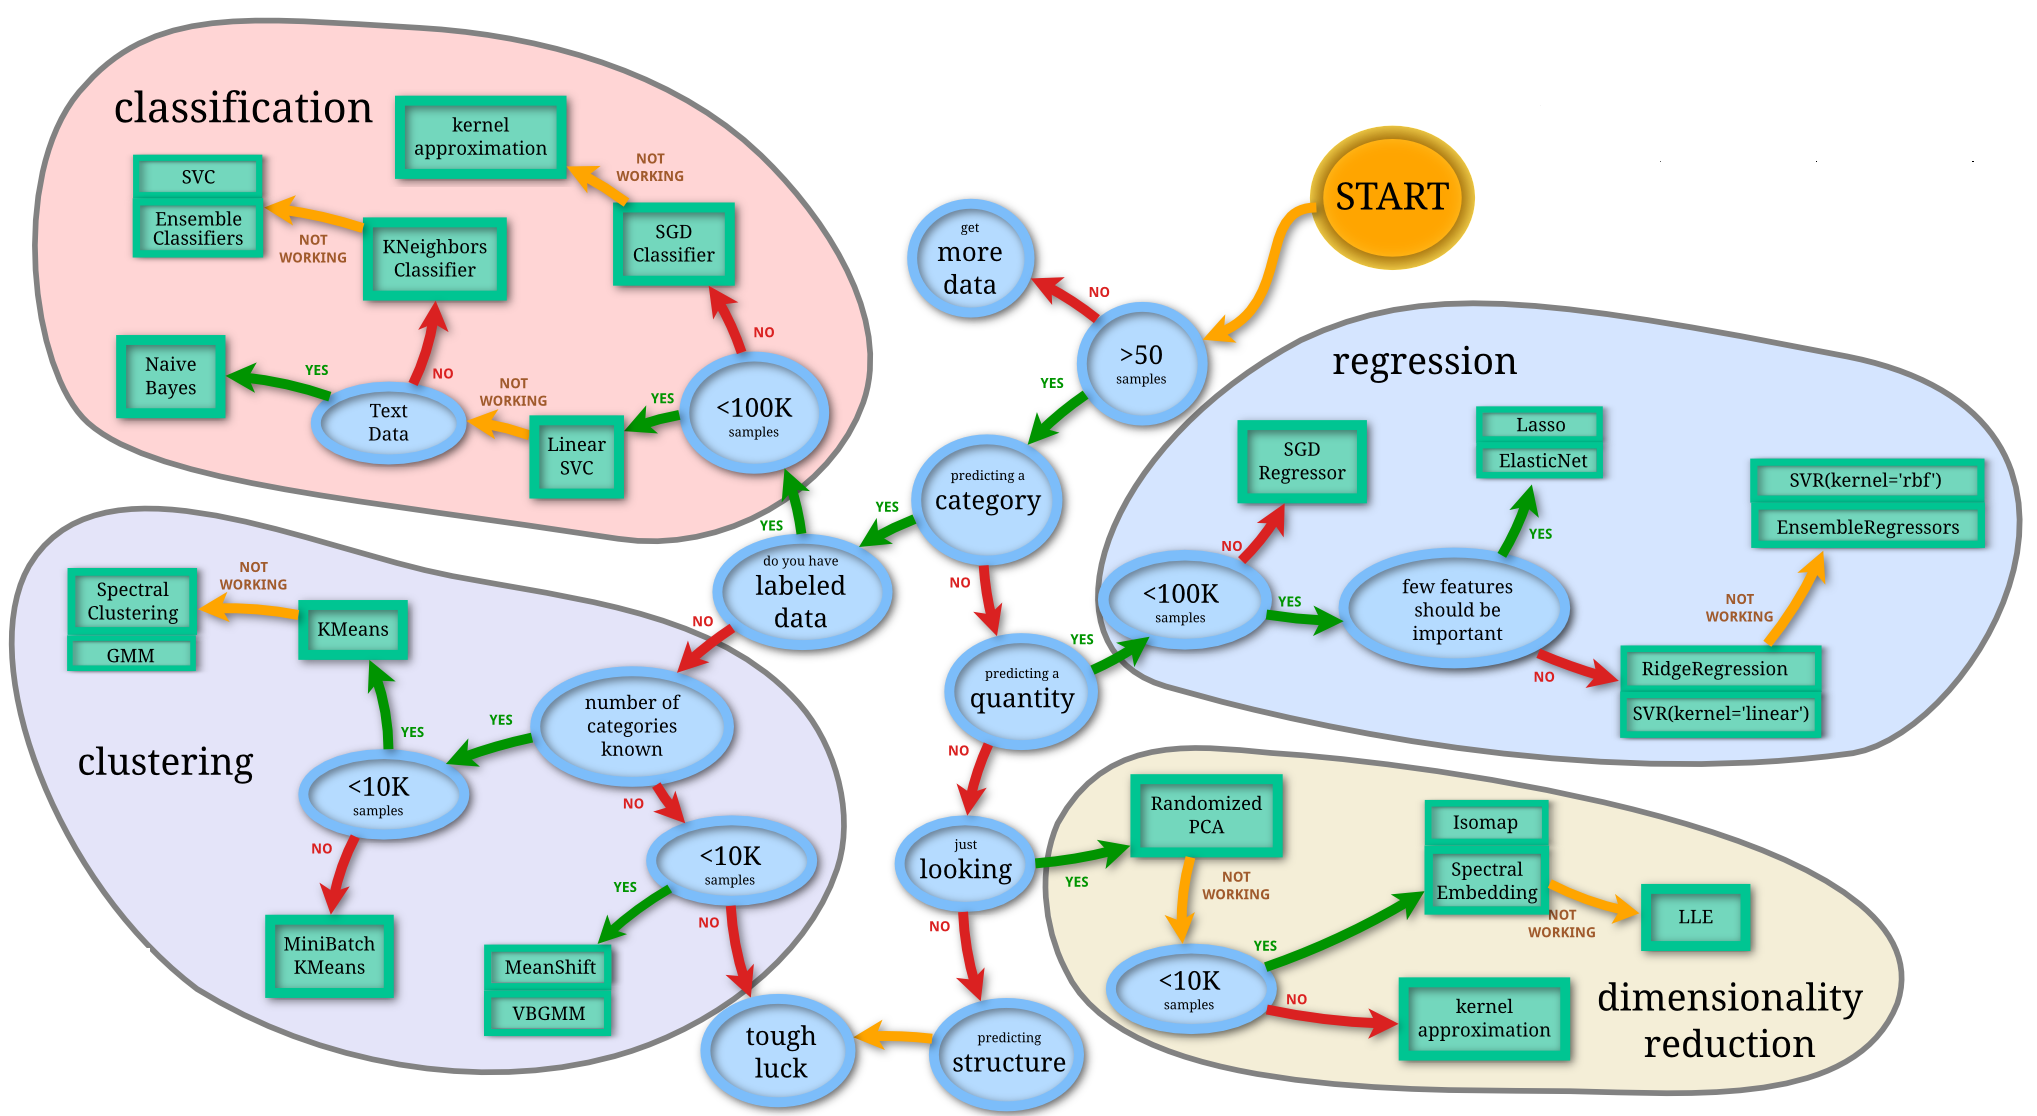
\includegraphics[width=17cm,height=12.2cm]{chapter2prime/fig2.png}
\end{center}
%légende de l'image
\caption{Data Analysis Techniques}
\label{analysis}
\end{figure}


\subsubsection{Data Representation}
Using visual representations to present data makes it easier to understand. Bar graphs, pie charts, line graphs, and histograms are an excellent way to illustrate data processing results. This section includes concepts and definitions, types of graphs
and charts \cite{cite12}.\\
~\\~\\
\textbf{\normalsize{Major Concepts and Definitions}}\\

Graphs and charts condense large amounts of information into easy-to-understand formats that clearly and effectively communicate important points. In selecting how best to present data,we have to think about the purpose of our graph or chart and what we want to present, then decide which variables we want to include and whether they should be expressed as frequencies, percentages, or categories.\\

When we decide what kind of graph or chart best illustrates our data, we should consider what type of data we are working with. Categorical data are grouped into non-overlapping categories (such as grade, race, and yes or no responses). Bar graphs, line graphs, and pie charts are useful for displaying categorical data. Continuous data are measured on a scale or continuum (such as weight or test scores). Histograms are useful for displaying continuous data.\\
~\\
\textbf{\normalsize{Types of Graphs and Charts}}\\

The main types of graphs, that can reduce complexity of unstructured data by transforming it into understandable form, are:\\
\begin{itemize}
\item \textbf{A bar graph} is composed of discrete bars  that represent different categories of data. The length or height of the bar is equal to the quantity within that category of data. Bar graphs are best used to compare values across categories.\\
\item \textbf{A pie chart} is a circular chart used to compare parts of the whole. It is divided into sectors that are equal in size to the quantity represented.\\
\item \textbf{A line graph} displays the relationship between two types of information, such as number of school personnel trained by year. They are useful in illustrating trends over time.\\
\item \textbf{A histogram} has connected bars that display the frequency or proportion of cases that fall within defined intervals or columns. The bars on the histogram can be of varying width and typically display continuous data.\\ 
\end{itemize}



%%%%%%%%%%%stop here
\newpage
\section{Study of The Existing}
In this section, we will establish a comparative study between already existing tools and take by the end which are the best tools that can be adopted in our project. 
\subsection{Existing Tools}
\subsubsection{Relational Database Management System}

\textbf{\normalsize{Drizzle:}}\\

Drizzle is a MySQL fork with a pluggable micro-kernel and with an emphasis of performance over compatibility. Like MySQL, Drizzle had a client/server architecture and uses SQL as its primary command language.

\begin{table}[H]
\caption{Drizzle Advantages and Disadvantages}
\begin{center}
\begin{tabularx}{17cm}{ |p{8.5cm}|X| } 
 \hline
 \textbf{Advantages} & \textbf{Disadvantages } \\ \hline
 $\bullet$ Better performance in modern machines \newline $\bullet$ Can run more than 4 hardware threads at once \newline $\bullet$ Drizzle can operate dynamic multi-statement SQL. Via the key word CONCURRENT, it can operate these statements in parallel. &  $\bullet$ Relational databases are not a suitable solution for large scale data management and analysis processing. \\ \hline

\end{tabularx}
\end{center}
\end{table}
\subsubsection{Non Relational Database Management System}
\textbf{\normalsize{MongoDB:}}\\

MongoDB is an open source NoSQL database that uses a document-oriented data model. Instead of using tables and rows as in relational databases, MongoDB is built on an architecture of collection and documents. Documents comprises sets of key-value pairs and are the basic unit of data in MongoDB. Collection contains sets of documents and function as the equivalent of relational database tables.\\



\begin{table}[H]
\caption{MongoDB Advantages and Disadvantages}
\begin{center}
\begin{tabularx}{17cm}{ |p{8.5cm}|X| } 
 \hline
 \textbf{Advantages} & \textbf{Disadvantages } \\ \hline
 $\bullet$ Horizontal scalability \newline $\bullet$ If the primary server goes down, the secondary server become the primary server without any human intervention\newline $\bullet$ It supports the common authentication mechanisms, such as LDAP, AD, and certificates. Users can connect to MongoDB over SSL and the data can be encrypted. \newline $\bullet$ MongoDB can be a cost effective solution because improves flexibility and reduces cost on hardware and storage. &  $\bullet$ No support transaction \newline $\bullet$ No join \newline $\bullet$ Memory limitation \\ \hline

\end{tabularx}
\end{center}
\end{table}
\newpage
\textbf{\normalsize{Cassandra:}}\\

Apache Cassandra is a free and open-source distributed NoSQL database management system designed to handle large amounts of data across many commodity servers, providing high availability with no single point of failure. Cassandra offers robust support for clusters spanning multiple data centers, with asynchronous masterless replication allowing low latency operations for all clients.\\



\begin{table}[H]
\caption{Cassandra Advantages and Disadvantages}
\begin{center}
\begin{tabularx}{17cm}{ |p{8.5cm}|X| } 
 \hline
 \textbf{Advantages} & \textbf{Disadvantages}  \\ \hline
  $\bullet$ Write speed \newline $\bullet$ Tunable consistency: Cassandra enables, on query-by-query basis, to decide how to handle potential issues. \newline $\bullet$ JVM based that means that Cassandra can easily integrate with other JVM based applications. \newline $\bullet$ CQL: is a familiar way of querying Cassandra, making the transition from an SQL based RDBMS to Cassandra less jarring. & $\bullet$ The Cassandra data storage layer is a key-value storage system. So, data should be modeled around the queries we want to surface, rather than around the structure of the data itself \newline $\bullet$ No Aggregations \newline $\bullet$ Unpredictable Performance due to no user-scheduled tasks \newline $\bullet$ Memory management is done by the language itself, not the application.  \\ \hline

\end{tabularx}
\end{center}
\end{table}
\subsubsection{Data Warehouse}
\textbf{\normalsize{Hive:}}\\

Hive is a data warehouse infrastructure build on Hadoop for providing data summarization query, and analysis. Hive gives an SQL-like interface to query data stored in various databases and file systems that integrate with Hadoop Traditional SQL queries must be implemented in the MapReduce java API to execute SQL applications and queries over distributed data.

\begin{table}[H]
\caption{Hive Advantages and Disadvantages}
\begin{center}
\begin{tabularx}{17cm}{ |p{8.5cm}|X| } 
 \hline
 \textbf{Advantages} & \textbf{Disadvantages}  \\ \hline
 $\bullet$ HIVE is very similar to SQL \newline $\bullet$ Data to be analyzed is stored in HDFS which provides all features like scalability, redundancy etc and SQL like query over data in Hadoop. \newline $\bullet$ Very useful for people who are not from Programming back ground (instead of writing 100 lines of MapReduce/Java program, same requirement can be done using 4 lines of a hive query) \newline $\bullet$ Used to handle structured data & $\bullet$ No real time access to data \newline $\bullet$ Updating data is complicated: \newline - Mainly because of using HDFS \newline - Can overwrite partitions \newline - Can add records \newline $\bullet$ High latency \newline $\bullet$ Slow  \\ \hline

\end{tabularx}
\end{center}
\end{table}

\subsubsection{Data Processing Frameworks}
\textbf{\normalsize{Hadoop:}}\\

Apache Hadoop is an open-source software framework used for distributed storage and processing of big data sets using the MapReduce programming model. It consists of computer clusters built from commodity hardware. All the modules in Hadoop are designed with a fundamental assumption that hardware failures are common occurrences and should be automatically handled by the framework.\\

The core of Apache Hadoop consists of a storage part, known as Hadoop Distributed File System (HDFS), and a processing part which is a MapReduce programming model. Hadoop splits files into large blocks and distributes them across nodes in a cluster. It then transfers packaged code into nodes to process the data in parallel. This approach takes advantage of data locality where nodes manipulate the data they have access to. This allows the dataset to be processed faster and more efficiently than it would be in a more conventional supercomputer architecture that relies on a parallel file system where computation and data are distributed via high-speed networking.\\

The base Apache Hadoop framework is composed of the following modules:
\begin{itemize}
\item Hadoop Common: contains libraries and utilities needed by other Hadoop modules
\item Hadoop Distributed File System (HDFS): is a distributed file-system that stores data on commodity machines, providing very high aggregate bandwidth across the cluster
\item Hadoop YARN: a resource-management platform responsible for managing computing resources in clusters and using them for scheduling of users' applications
\item Hadoop MapReduce: an implementation of the MapReduce programming model for large scale data processing
\end{itemize}




\begin{table}[H]
\caption{Hadoop Advantages and Disadvantages}
\begin{center}
\begin{tabularx}{17cm}{ |p{8.5cm}|X| } 
 \hline
\textbf{Advantages} & \textbf{Disadvantages } \\ \hline
 $\bullet$ Scalable: it can store and distribute very large data sets across hundreds of inexpensive severs that operate in parallel \newline $\bullet$ Cost effective \newline $\bullet$ Flexible \newline $\bullet$ Fast \newline $\bullet$ Resilient to failure & $\bullet$ Security Concerns \newline $\bullet$ Vulnerable by nature \newline $\bullet$ Not fit for small data \newline $\bullet$ Potential Stability Issues \newline $\bullet$ General Limitation  \\ \hline

\end{tabularx}
\end{center}
\end{table}
\textbf{\normalsize{Blobseer:}}\\

BlobSeer is a large-scale distributed storage service that addresses advanced data management requirements resulting from ever-increasing data sizes. It is centered around the idea of leveraging versioning for concurrent manipulation of binary large objects in order to efficiently exploit data-level parallelism and sustain a high throughput despite massively parallel data access.\\



\begin{table}[H]
\caption{Blobseer Advantages and Disadvantages}
\begin{center}
\begin{tabularx}{17cm}{ |p{8.5cm}|X| } 
 \hline
 \textbf{Advantages} & \textbf{Disadvantages}  \\ \hline
 $\bullet$ A single process that writes on a large file (> 20 GB) \newline $\bullet$ Processes that read the same parts of a single file at the same time \newline $\bullet$ Processes that write in the same large file \newline $\bullet$ Fine-grained write access \newline $\bullet$ Good horizontal scalability \newline $\bullet$ Applicable to Hadoop Map/Reduce applications (it comes with a HDFS compatibility layer) & $\bullet$ The version manager is a single point of failure, and hot spot (in the critical path for both reads or writes) \newline $\bullet$ Metadata distribution in a distributed tree may cause high latency as the size of the tree grows \newline $\bullet$ No eviction for old version, causing decreasing performance over time  \\ \hline

\end{tabularx}
\end{center}
\end{table}

\textbf{\normalsize{Spark Apache:}}\\

Apache Spark is a fast and general engine for large-scale data processing. Spark powers aa stack of libraries including SQL and Data Frames, MLlib for machine learning, GraphX, and spark Streaming.\\

Spark extends its predecessors with in-memory processing. Its Resilient Distributed Dataset (RDD) abstraction enables developers to materialize any point in a processing pipeline into memory across the cluster, meaning that future steps that want to deal with the same data set need not recompute it overload it from disk.\\

Sparks runs on Hadoop, Mesos, standalone, or in the cloud. It can access diverse data sources including HDFS, Cassandra and HBase.

\begin{table}[H]
\caption{Spark Advantages and Disadvantages}
\begin{center}
\begin{tabularx}{17cm}{ |p{8.5cm}|X| } 
 \hline
 \textbf{Advantages} & \textbf{Disadvantages}  \\ \hline
 $\bullet$ Faster batch processing than MapReduce. Spark executes batch-processing jobs 10 to 100 times faster than MapReduce \newline $\bullet$ Spark comes with GraphX, a distributed graph system \newline $\bullet$ Spark is ideal for iterative processing, interactive processing and event stream processing \newline $\bullet$ Spark can run on Hadoop alongside other tools in the Hadoop ecosystem including Hive & $\bullet$ Spark is still working out bugs as it matures.\\ \hline

\end{tabularx}
\end{center}
\end{table}
\subsection{Technical Specification}
Spark Apache, as a Bigdata provessing tool, provides mainly four API in four different programming languages which are: Java, Scala, R and Python. Java is a programming language that uses JVM (Java Virtual Machine) which make it no suitable for processing a large scale of data. R is interpreted programming language oriented to Data Science users, but it is made for executing some specified operations and not making a whole application or service that can be used through other applications. So, we have to choose between Scala and Python programming language.\\

Table \ref{cmp} is an established comparison between Python and Scala as two programming languages applied on Apche Spark. 
~\\ ~\\ ~\\
\begin{table}[H]
\caption{Scala Vs. Python on Apache Spark}
\begin{center}
\begin{tabularx}{17cm}{ |p{2.8cm}|X|X| } 
 \hline
 \textbf{Criteria} & \textbf{Scala} & \textbf{Python} \\ \hline
  Learning curve & Scala’s syntax makes it difficult to master & Python is comparatively easier to learn because of its syntax and standard libraries.\\ \hline
  Concurrence & Scala allows developers to write efficient, readable and maintainable services without dangling the program code into an unreadable cobweb of call-backs. & Python does support heavyweight process forking using uwsgi but it does not support true multithreading.\newline
(When using Python for Spark, irrespective of the number of threads the process has only one CPU is active at a time for a Python process. This helps get around with one process per CPU core but the downfall to this is, that whenever a new code is to be deployed, more processes need to restart and it also requires additional memory overhead. Scala is more efficient and easy to work with in these aspects.)\\ \hline
  Type safety & Statically typed language (Scala is a statically typed language through it appears like a dynamically typed language because of the classy type inference mechanism. Being a statically typed language, Scala still provides the compiler to catch compiler to catch compile time errors) & Dynamically typed language (Developers often face difficulties after modifying Python program as it creates more bugs than fixing the older ones.\\ \hline
  Performance & Scala is faster when there are less number of cores. As the number of cores increases, the performance advantage of Scala starts to dwindle) & For a big number of cores, Python is faster than Scala and present a better execution time \\ \hline
  Ease of use & Verbose language & Less verbose and easier to use than Scala\\ \hline
  Advanced \newline features & Has several existential types, macros and implicits but lacks good visualization and local data transformations.
(The arcane syntax of Scala might make it difficult to experiment with the advanced features which might be incomprehensible to the developers. / Scala lacks good visualization and local data transformations.) & Has several libraries for machine Learning and Natural language processing.
(Python has sufficient data science tools and libraries for machine learning, SparkMLlib / Python Spark streaming support is not advanced and mature like Scala)\\ \hline
  Documentation/\newline community &Scala belongs to the tier1 (classified by \#tags in stack overflow and GitHub) & Python belongs also to the tier1. If we consider documentation of the machine learning and statistics frameworks, the Python data science community is more mature.\\ \hline
\end{tabularx}
\end{center}
\label{cmp}
\end{table}
\newpage
\section{Technical Review}
As we have, in our case, a huge amount of unstructured data, the most suitable framework to process advanced and complex analytical algorithms on that data is \textbf{Spark Apache}, as it provides a rich libraries and features that can be adapted to our work. Spark Apache is well performed with \textbf{Python programming language}. In fact, Python provides a variety of tools to present data structure and a plenty of libraries for data mining and data science. Data storage needs also a well performing tool to maintain a large scale of data well maintained for data processing and data-keep-in-security, \textbf{Hadoop Distributed File System (HDFS)} is file system that matches perfectly with Spark Apache. 
 

\section*{Conclusion} 

Throughout this chapter, we explained some theoretical concepts that are essential to understand what follows. We have also established an existing study on which we compared the already existing tools for manufacturing Bigdata. Based on the studied solutions, we will be able to set our project requirements. But before going through this step, we have to define how the chosen tools work. That is the purpose of the coming chapter.
\chapter{Parallel Architectures}
\label{Chapter2prime}
After establishing a comparative study of the existing, this chapter is meant to define the main features and the architecture of both Hadoop Distributed File System and Apache spark framework.  

\section{The Hadoop Distributed File System}

The Hadoop Distributed File System (HDFS) is a distributed file system designed to run on service hardware. Unlike other distributed systems, HDFS is highly fault-tolerant and designed using low-cost hardware. HDFS holds very large amount of data and provides easier access. To store such huge data, the files are stored across multiple machines. These files are stored in a way to rescue the system from possible data losses in case of failure. HDFS also makes applications available to parallel processing \cite{cite14}.\\

\subsection{Features of HDFS:}
HDFS provides a plenty of functionalities and features that make processing and storing huge datasets easier and more secure. To better understand HDFS, following will explain its goals and assumptions: \\

\textbf{\normalsize{Hardware Failure}}\\

Hardware failure is the norm rather than the exception in HDFS architecture. A node may consist of many server machines, each storing part of the file system's data. The fact that there are a big number of components and that each component has a non-trivial possibility of failure means that some component of HDFS is always non-functional. Thus, quick detection of faults and automatic recovery is a core architectural goal of HDFS.\\

\textbf{\normalsize{Streaming Data Access}}\\

Applications' datasets that run on HDFS need streaming to access. They are not general purpose applications that classically run on general purpose file systems. HDFS is designed more for batch processing rather than interactive use. The emphasis is on high amount of data access rather than low latency of data access. POSIX imposes many hard requirements that are not needed for applications that are targeted for HDFS. POSIX semantics in a few key areas has been traded to rise data throughput rates.\\

\textbf{\normalsize{Large Datasets}}\\

A usual file in HDFS is huge in size. HDFS is designed, then, to support large files. It should provide high aggregate data bandwidth and scale to hundreds of nodes in a single cluster. It should support tens of millions of files in a single instance.\\

\textbf{\normalsize{Simple Coherency Model}}\\

HDFS applications need a "write once read many" access model for files. A file once created, written, and closed needs not to be changed. This assumption simplifies data coherency issues and enables high amount data access. A Map-Reduce application or a web based application fits perfectly with this model. There is a plan to support appending-writes to files in the future.\\

\textbf{\normalsize{Computing Data Mode}}\\

A computation requested by an application is much more efficient if it is executed near the data it operates on. This is especially true when the size of the dataset is huge. This minimizes network congestion and increases the overall throughput of the system. The assumption is that it is often better to migrate the computation closer to where the data is located rather than moving the data to where the application is running. HDFS provides interfaces for applications to move themselves closer to where the data is located.\\

\textbf{\normalsize{Portability Across Hardware and Software Platforms}}\\

HDFS has been designed to be easily portable from one platform to another. This helps extensive adoption of HDFS as a platform of choice for a large number of applications.

 
\subsection{HDFS Architecture:}

HDFS follows the master/slave architecture and it has the following elements. Figure \ref{hdfsarch} given below is the architecture of a Hadoop File System \cite{cite15}.

\begin{figure}[H]
\begin{center}
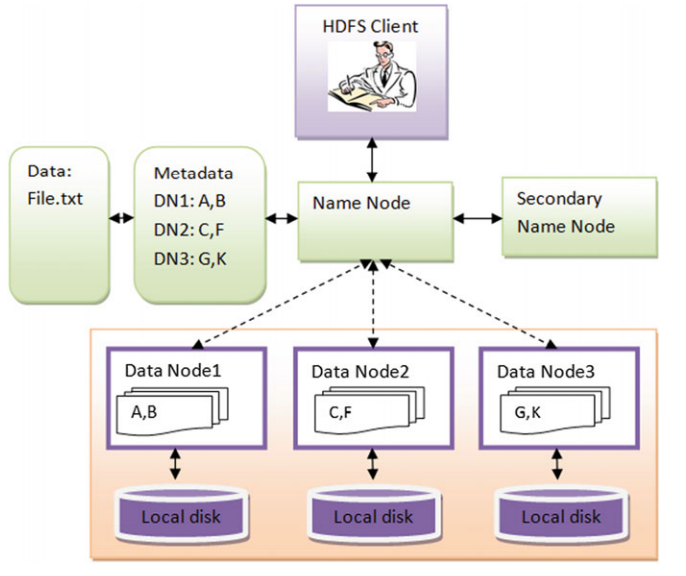
\includegraphics[width=13.8cm,height=8cm]{chapter2/fig2.png}
\end{center}
%légende de l'image
\caption{HDFS Architecture}
\label{hdfsarch}
\end{figure}

\begin{itemize}
\item \textbf{NameNode:} The namenode is the commodity hardware that contains the operating system and the namenode software. It is a software that can be run on commodity hardware. The system having the namenode acts as the master server and it does the following tasks: 
\begin{itemize}
\item Manages the file system namespace.
\item Regulates client's access to files.
\item It also executes file system operations such as renaming, closing, and opening files and directories.
\end{itemize}
A secondary namenode is defined as a backup name node in case of failure.
\item \textbf{DataNodes:} The datanode is a commodity hardware having an operating system and datanode software. For every node (Commodity hardware/System) in a cluster, there will be a datanode. These nodes manage the data storage of their system. 
\begin{itemize}
\item Datanodes perform read-write operations on the file systems, as per client request.
\item They also perform operations such as block creation, deletion, and replication according to the instructions of the namenode. 
\end{itemize}

\item \textbf{Blocks:} Generally the user data is stored in the files of HDFS. The file in a file system will be divided into one or more segments and stored in individual data nodes. These file segments are called as blocks. In other words, the minimum amount of data that HDFS can read or write is called a Block. HDFS configuration set the block size. Otherwise, it will be defined by default.

\item \textbf{HDFS Client:} User applications access the file system using the HDFS client library. HDFS supports operations to read, write and delete files, and operations to create and delete directories. The user references files and directories by paths in the namespace. The user application does not need to know that file blocks are on different servers \cite{cite13}. When an application reads a file, the HDFS client first asks the namenode for the list of datanodes that host blocks replicas of the file. It then contacts a datanode directly and requests the transfer of the desired block. When a client writes, it asks the namenode to choose datanodes to host replicas of the first block of the file. The client organizes a pipeline from node to node and sends the data. When the first block is filled, the client requests new datanodes to be chosen to host replicas of the next block. A new pipeline is organized, and the client sends the further bytes of the file. Each choice of datanodes is likely to be different. The interactions among the client, the namenode and the datanodes are illustrated in figure \ref{interaction}.
\end{itemize} 


\begin{figure}[H]
\begin{center}
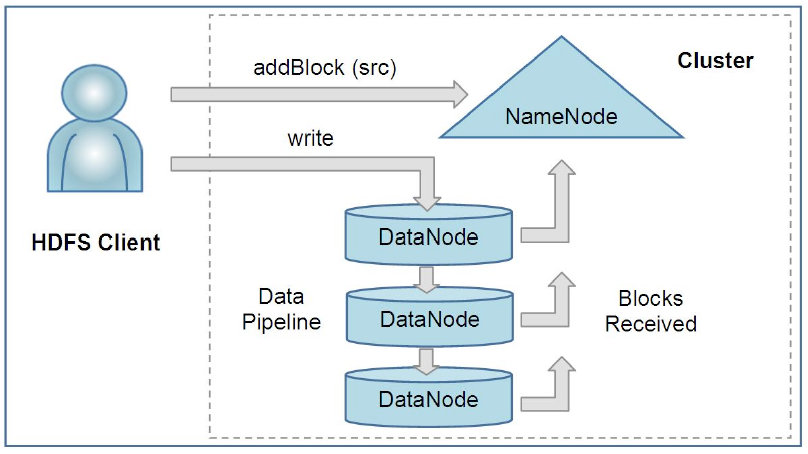
\includegraphics[width=13.5cm,height=6cm]{chapter2/fig1.png}
\end{center}
%légende de l'image
\caption{Interaction between a HDFS Client and Cluster}
\label{interaction}
\end{figure}


\subsection{The File System Namespace}

HDFS supports a traditional hierarchical file organization. A user or an application can create directories and store files inside these directories. The file system namespace hierarchy is similar to most other existing file systems; one can create and remove files, move a file from one directory to another, or rename a file.\\

The namenode maintains the file system namespace. Any change to the file system namespace or its properties is recorded by the namenode. An application can specify the number of replicas of a file that should be maintained by HDFS. The number of copies of a file is called the replication factor of that file. This information is stored by the nameode \cite{cite23}.\\

\subsubsection{File Read and Write}

An application adds data to HDFS by creating a new file and writing the data to it. After the file is closed, the bytes written cannot be altered or removed except that new data can be added to the file by reopening the file for append. HDFS implements a single writer, multiple reader model.\\ 

The HDFS client that opens a file for writing is granted a lease for the file; no other client can write to the file. The writing client periodically renews the lease by sending a heartbeat to the namenode. When the file is closed, the lease is revoked. \\

An HDFS file consists of blocks. When there is a need for a new block, the namenode allocates a block with a unique block ID and determines a list of datanodes to host replicas of the block. The datanodes form a pipeline, the order of which minimizes the total network distance from the client to the last datanode. Bytes are pushed to the pipeline as a sequence of packets. The bytes that an application writes first buffer at the client side. After a packet buffer is filled, the data are pushed to the pipeline. The next packet can be pushed to the pipeline before receiving the acknowledgement for the previous packets. The number of outstanding packets is limited by the outstanding packets window size of the client \cite{cite23}. After data are written to an HDFS file, HDFS does not provide any guarantee that data are visible to a new reader until the file is closed.

\begin{figure}[!h]
\begin{center}
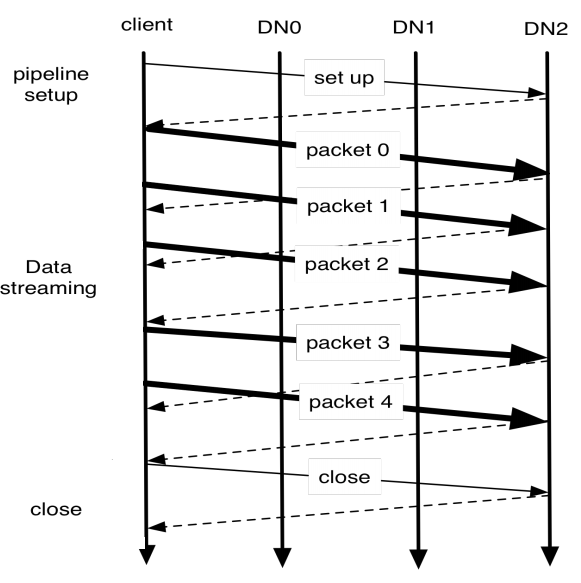
\includegraphics[width=9.5cm,height=9cm]{chapter2prime/pipeline.png}
\end{center}
%légende de l'image
\caption{Data Pipeline During Block Construction}
\label{pipline}
\end{figure}

If no error occurs, block construction goes through three stages as shown in figure \ref{pipline} illustrating a pipeline of three datanodes and a block of five packets. In the picture, bold lines represent data packets, dashed lines represent acknowledgment messages, and thin lines represent control messages to setup and close the pipeline. Vertical lines represent
activity at the client and the three datanodes where time proceeds from top to bottom.\\

When a client opens a file to read, it fetches the list of blocks and the locations of each block replica from the
namenode. The locations of each block are ordered by their distance from the reader. When reading the content of a block,
the client tries the closest replica first. If the read attempt fails, the client tries the next replica in sequence. A read may fail if the target datanode is unavailable, the node no longer hosts a replica of the block, or the replica is found to be corrupt when checksums are tested. HDFS permits a client to read a file that is open for writing. When reading a file open for writing, the length of the last
block still being written is unknown to the namenode. In this case, the client asks one of the replicas for the latest length before
starting to read its content \cite{cite23}.\\


\subsubsection{Replica Placement}
The placement of replicas is critical to HDFS reliability and performance. Optimizing replica placement distinguishes HDFS from most other distributed file systems. The purpose of a rack-aware replica placement policy is to improve data reliability, availability, and network bandwidth utilization.\\

Large HDFS instances run on a cluster of computers that commonly spread across many racks. Communication between two nodes in different racks has to go through switches. In most cases, network bandwidth between machines in the same rack is greater than network bandwidth between machines in different racks.\\

The namenode determines the rack ID each datanode belongs to. A simple policy is to place replicas on unique racks. This prevents losing data when an entire rack. This policy evenly distributes replicas in the cluster, which makes it easy to balance load on component failure. However, this policy increases the cost of writes because a write needs to transfer blocks to multiple racks.
\subsubsection{Communication Protocols}
All HDFS communication protocols are layered on top of the TCP/IP protocol. A client
establishes a connection to a configurable TCP port on the namenode machine. It talks
the ClientProtocol with the namenode. The datanodes talk to the namenode using the
datanode Protocol. A Remote Procedure Call (RPC) abstraction wraps both the Client
Protocol and the datanode Protocol. By design, the namenode never initiates any RPCs. Instead, it only responds to RPC requests issued by datanodes or clients.

\section{Spark: Framework for Parallel Execution}
Apache Spark is a lightning-fast cluster computing technology, designed for fast computation. It is based on Hadoop Map-Reduce and it extends the Map-Reduce model to efficiently use it for more types of computations, which includes interactive queries and stream processing. The main feature of Spark is its in-memory cluster computing that increases the processing speed of an application.\\

Spark is designed to cover a wide range of workloads such as batch applications, iterative algorithms, interactive queries and streaming. Apart from supporting all these workload in a respective system, it reduces the management burden of maintaining separate tools.\\

\subsection{Features of Spark Apache}
\begin{itemize}
\item \textbf{Speed:} Spark helps to run an application in Hadoop cluster, up to 100 times faster in memory, and 10 times faster when running on disk. This is possible by reducing number of read/write operations to disk. It stores the intermediate processing data in memory.
\item \textbf{Supports multiple languages:} Spark provides built-in APIs in Java, Scala, or Python. Therefore, we can write applications in different languages. Spark comes up with 80 high-level operators for interactive querying.
\item \textbf{Advanced Analytics:} Spark not only supports "Map" and "Reduce". It also supports SQL queries, Streaming data, Machine learning (ML), and Graph algorithms.\\
\end{itemize}

\subsection{Components of Spark}

Figure \ref{component} shows the different components of Spark \cite{cite1}.

\begin{figure}[!ht]
\begin{center}
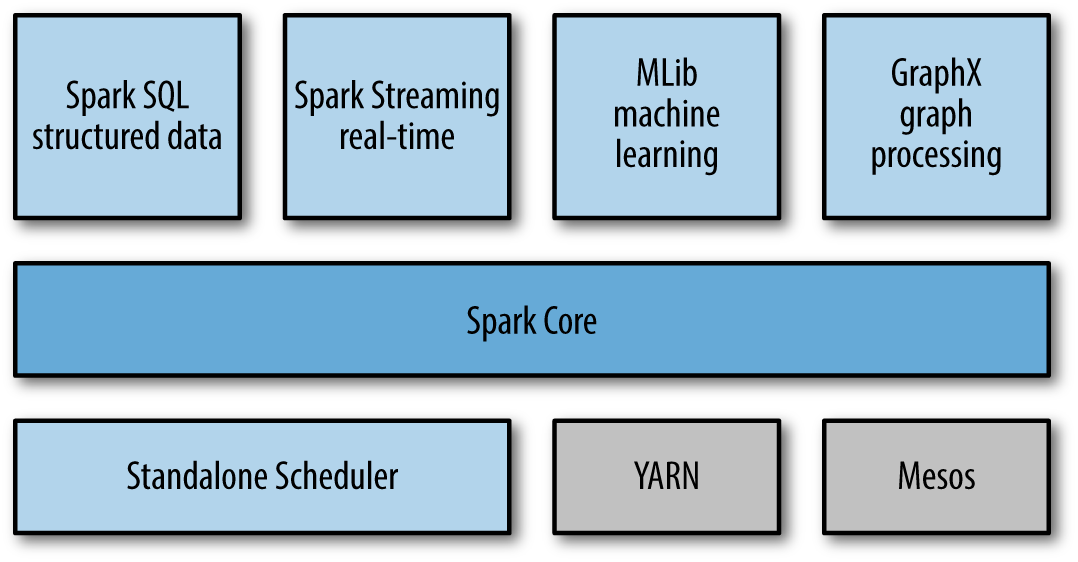
\includegraphics[width=13cm,height=5cm]{chapter2/fig3.png}
\end{center}
%légende de l'image
\caption{The Spark Stack}
\label{component}
\end{figure}



\begin{itemize}
\item \textbf{Apache Spark Core:} Spark Core is the underlying general execution engine for spark platform that all other functionality is built upon. It provides In-Memory computing and referencing datasets in external storage systems.
\item \textbf{Spark SQL:} Spark SQL is a component on top of Spark Core that introduces a new data abstraction called SchemaRDD, which provides support for structured and semi-structured data.
\item \textbf{Spark Streaming:} Spark Streaming leverages Spark Core's fast scheduling capability to perform streaming analytics. It ingests data in mini-batches and performs RDD (Resilient Distributed Datasets) transformations on those mini-batches of data.
\item \textbf{MLlib (Machine Learning Library):} MLlib is a distributed machine learning framework above Spark because of the distributed memory-based Spark architecture. Spark MLlib is nine times as fast as the Hadoop disk-based version.
\item \textbf{GraphX:} GraphX is a distributed graph-processing framework on top of Spark. It provides an API for expressing graph computation that can model the user-defined graphs by using Pregel abstraction API. It also provides an optimized runtime for this abstraction.\\
\end{itemize}

\subsection{Resilient Distributed Datasets}

Resilient Distributed Datasets (RDD) is a fundamental data structure of Spark. It is an immutable distributed collection of objects. Each dataset in RDD is divided into logical partitions, which may be computed on different nodes of the cluster. RDDs can contain any type of Python, Java, or Scala objects, including user-defined classes \cite{cite1}.\\

Formally, an RDD is a read-only, partitioned collection of records. RDDs can be created through deterministic operations on either data on stable storage or other RDDs. RDD is a fault-tolerant collection of elements that can be operated on in parallel. There are two ways to create RDDs: parallelizing an existing collection in the driver program, or referencing a dataset in an external storage system, such as a shared file system, HDFS, HBase, or any data source offering a Hadoop Input Format.\\

Spark makes use of the concept of RDD to achieve faster and efficient MapReduce operations. Let us first discuss how MapReduce operations take place and why they are not so efficient.

\subsection{Map Reduce} 

Map-Reduce is a technique that is widely adopted for processing and generating large datasets with a parallel, distributed algorithm on multiple clusters. It allows users to write parallel computations, using a set of high-level operators, without having to worry about work distribution and fault tolerance.\\

Unfortunately, in most current frameworks, the only way to reuse data between computations is to write it to an external stable storage system. Although this framework provides numerous abstractions for accessing a cluster's computational resources, users still want more.\\

Both Iterative and Interactive applications require faster data sharing across parallel jobs. Data sharing is slow in Map-Reduce due to replication, serialization, and disk input/output (IO). Regarding storage system, most of the Hadoop applications, they spend most of the time doing HDFS read-write operations.
\begin{itemize}
\item \textbf{Iterative Operations on Map Reduce:} Reuse intermediate results across multiple computations in multi-stage applications. Figure \ref{iterative} explains how the current framework works, while doing the iterative operations on Map-Reduce. This incurs substantial overheads due to data replication, disk IO, and serialization, which makes the system slow.

\begin{figure}[H]
\begin{center}
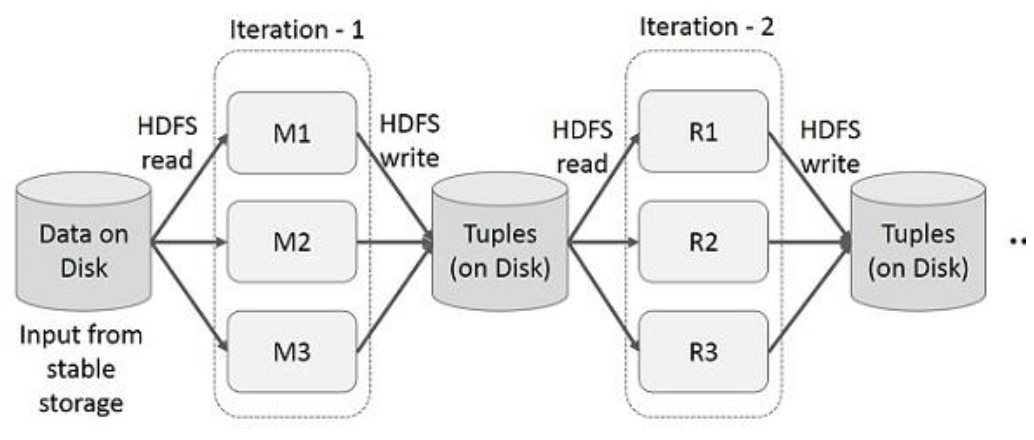
\includegraphics[width=14cm,height=6cm]{chapter2/fig4.png}
\end{center}
%légende de l'image
\caption{Iterative Operations on MapReduce}
\label{iterative}
\end{figure}

\item \textbf{Interactive Operations on MapReduce:} User runs ad-hoc queries on the same subset of data. Each query will do the disk I/O on the stable storage, which can dominates application execution time. Figure \ref{interactive} explains how the current framework works while doing the interactive queries on MapReduce.

\begin{figure}[H]
\begin{center}
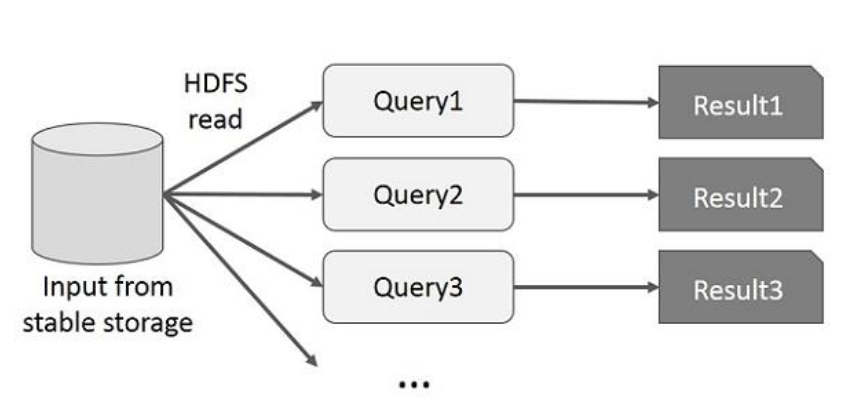
\includegraphics[width=14cm,height=6cm]{chapter2/fig5.png}
\end{center}
%légende de l'image
\caption{Interactive operations on MapReduce}
\label{interactive}
\end{figure}

\item \textbf{Data Sharing using Spark RDD:} Data sharing is slow in Map-Reduce due to replication, serialization, and disk IO. Most of the Hadoop applications, they spend most of the time doing HDFS read-write operations. Recognizing this problem, researchers developed a specialized framework called Apache Spark. The key idea of spark is Resilient Distributed Datasets (RDD); it supports in-memory processing computation. This means, it stores the state of memory as an object across the jobs and the object is sharable between those jobs. Data sharing in memory is 10 to 100 times faster than network and Disk.
Let us now try to find out how iterative and interactive operations take place in Spark RDD.

\item \textbf{Iterative Operations on RDD Spark:} Figure \ref{RDD1} shows the iterative operations on Spark RDD. It will store intermediate results in a distributed memory instead of Stable storage (Disk) and make the system faster.



\begin{figure}[H]
\begin{center}
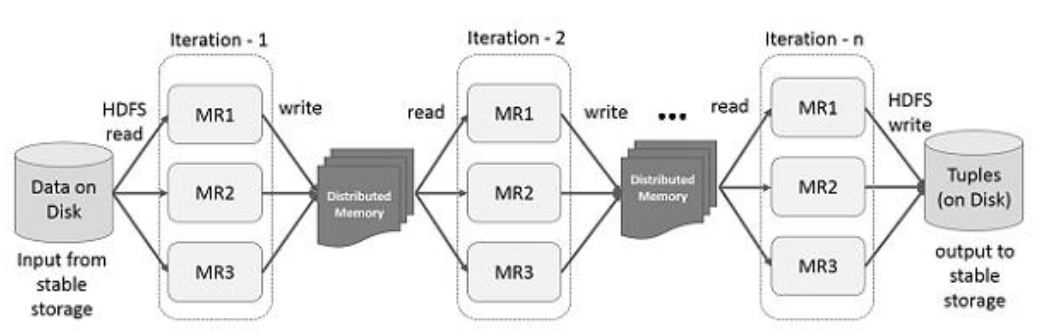
\includegraphics[width=16cm,height=6.5cm]{chapter2/fig6.png}
\end{center}
%légende de l'image
\caption{Iterative operations on Spark RDD}
\label{RDD1}
\end{figure}



\item \textbf{Interactive Operation on Spark RDD:} Figure \ref{RDD2} shows interactive operations on Spark RDD. If different queries are run on the same set of data repeatedly, this particular data can be kept in memory for better execution times.\\

\begin{figure}[H]
\begin{center}
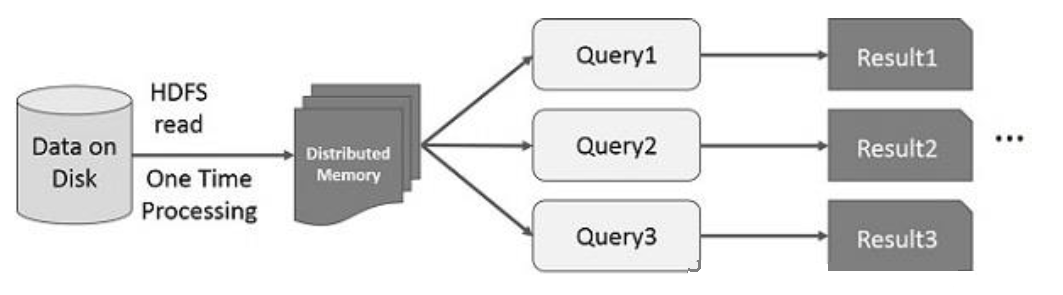
\includegraphics[width=14cm,height=6cm]{chapter2/fig7.png}
\end{center}
%légende de l'image
\caption{Interactive operations on Spark RDD}
\label{RDD2}
\end{figure}

\end{itemize}

\subsection{Spark Architecture}

Spark applications run as independent sets of processes on a cluster, coordinated by a SparkContext object in a main program called the driver program. Specifically, to run on a cluster, the SparkContext can connect to several types of cluster managers; either Spark's own standalone cluster manager, Mesos or YARN, which allocate resources across applications. Once connected, Spark acquires executors on nodes in the cluster, which are processes that run computations and store data for the application. Next, it sends the application code to the executors. Finally, SparkContext sends tasks to the executors to run. Figure \ref{driver} shows how this architecture works.\\
\begin{figure}[!ht]
\begin{center}
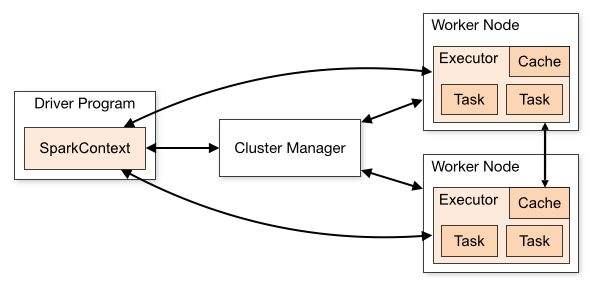
\includegraphics[width=14cm,height=7cm]{chapter2/fig8.png}
\end{center}
%légende de l'image
\caption{Spark Architecture}
\label{driver}
\end{figure}

There are several useful things to note about this architecture:\\
\begin{itemize}
\item Each application gets its own executor processes, which stay up for the duration of the whole application and run tasks in multiple threads. This has the benefit of isolating applications from each other, on both the scheduling side (each driver schedules its own tasks) and executor side (tasks from different applications run in different JVMs). However, it also means that data cannot be shared across different Spark applications (instances of SparkContext) without writing it to an external storage system.
\item Spark is agnostic to the underlying cluster manager. As long as it can acquire executor processes, and these communicate with each other, it is relatively easy to run it even on a cluster manager that also supports other applications.
\item The driver program must listen for and accept incoming connections from its executors throughout its lifetime. As such, the driver program must be network addressable from the worker nodes.
\item Because the driver schedules tasks on the cluster, it should be run close to the worker nodes, preferably on the same local area network. If we'd like to send requests to the cluster remotely, it's better to open an RPC to the driver and have it submit operations from nearby than to run a driver far away from the worker nodes.
\end{itemize}

\section*{Conclusion}

After describing, theoretically, our chosen big data manufacturing tools, in the next
chapter, we are going to start the application development step by, first specifying the requirements of the application that we opt to implement.
\chapter{Requirements Analysis and Specification}
\label{Chapter3} 
Defining correctly the requirements that our work is asked to satisfy, is one of the most important steps during our project development. During this chapter, we will analyze requirements within describing those that are functional and those that are non-functional. Then in a second section, we will define the dynamic behavior of the system, by introducing the interaction between its different actors and the entire system. 
\section{Requirement Analysis}
\subsection{Identifying Actors}
An actor is a role played by an external entity which interacts directly with the studied system. In our case, we have two types of external actors that are matched directly with our system: \\
\begin{itemize}
\item \textbf{Administrator:} is an external entity that manage the whole system and customize users roles.\\
\item \textbf{Client:} is the entities that the application should provide a service for. First, ask for a permission to access to the application then operate algorithms.\\  
\end{itemize}




Both of these actors have some functionalities in common, such as running mining algorithms. So, we can represent the relation between them as an inheritance. Figure \ref{actors} represent this relation:

\begin{figure}[!ht]
\begin{center}
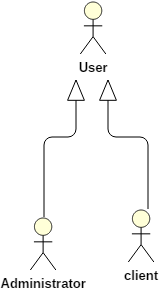
\includegraphics[width=4.75cm,height=4.5cm]{chapter3/actors.png}
\end{center}
\caption{Inheritance Relationship between Actors}
\label{actors}
\end{figure}


\subsection{Functional requirements}

The delivered application consists on designing and implementing Client / Server application that should satisfy the specific functionalities listed below:
\begin{itemize}
\item The system must offer to the user the possibility to load big data from different sources into HDFS. 
\item The system must engineer the best implementation of the required algorithms in order to perform the best execution time and memory management.
\item The user is not coming from An IT background; all command lines should be hidden behind a Graphical User Interface. 
\item The system allows user to apply, on large volume of data, several data mining algorithms such as:
\begin{itemize}
\item Principal components analysis 
\item Linear Model
\item K-Means
\end{itemize}
\item The User should be able to visualize algorithm results in different interactive forms (Charts, Graphics, data visualizations, grids …)
\item The application should provide a users management feature in order to affect different roles for every user category.
\item The application should provide for the administrator user the ability to log every operation lunched by the client. This functionality enables reporting issues.
\item This application should offer the ability for every client to ask for a registration. After administrator permission, he would be able to access and process algorithm on his loaded data.
\end{itemize}
\subsection{Non-functional requirements}

While achieving the functional requirements, the solution should satisfy the following non functional requirements:
\begin{itemize}
\item \textbf{Scalability:} The modularity and extensibility of the application architecture in case of the addition of new features or new algorithm. In our case, when the size or volume of data becomes larger or the number of servers increase, the application should guarantee a regular behaviour. We can also add new algorithms in case of necessity. 
\item \textbf{Ease of use:} As users are almost from a non-IT background, the application must have a user-friendly and ergonomic interface.
\item \textbf{Security:} The data storage should be far from being accessed by an unwanted user. Every operation of access should be preceded by an authentication. Data storage servers should be able to provide availability of the data when required.
\item \textbf{Robustness :} Robustness is the system's ability to cope and deal with errors that may occur during the system's execution. It is an important criterion to the system. In fact, the application should ensure a good error management when displaying data or processing. Accidents
like a server crash or failure should be handled in a safe way and error. Moreover, error messages should be precise and correct.

\item \textbf{Documentation:} The solution should be well-documented in order to provide the best use for the costumer.
\end{itemize}
\section{Requirement Specification}
To have a better understanding of the required needs, we will model them in a formal way using use case and activity diagrams.
\subsection{System Use Case}
The use case diagram captures the behaviour of a software system. This diagram describes
the various actions, which can be made by an outside user. It splits the feature of the system into coherent units, the use cases, having a sense for the actors.\\

The figure \ref{user} shows the general use case diagram that includes the common functionalities for all components.\\

In order to clarify the previous diagram, we present a detailed description of the use case in the table \ref{description}.
\begin{figure}[H]
\begin{center}
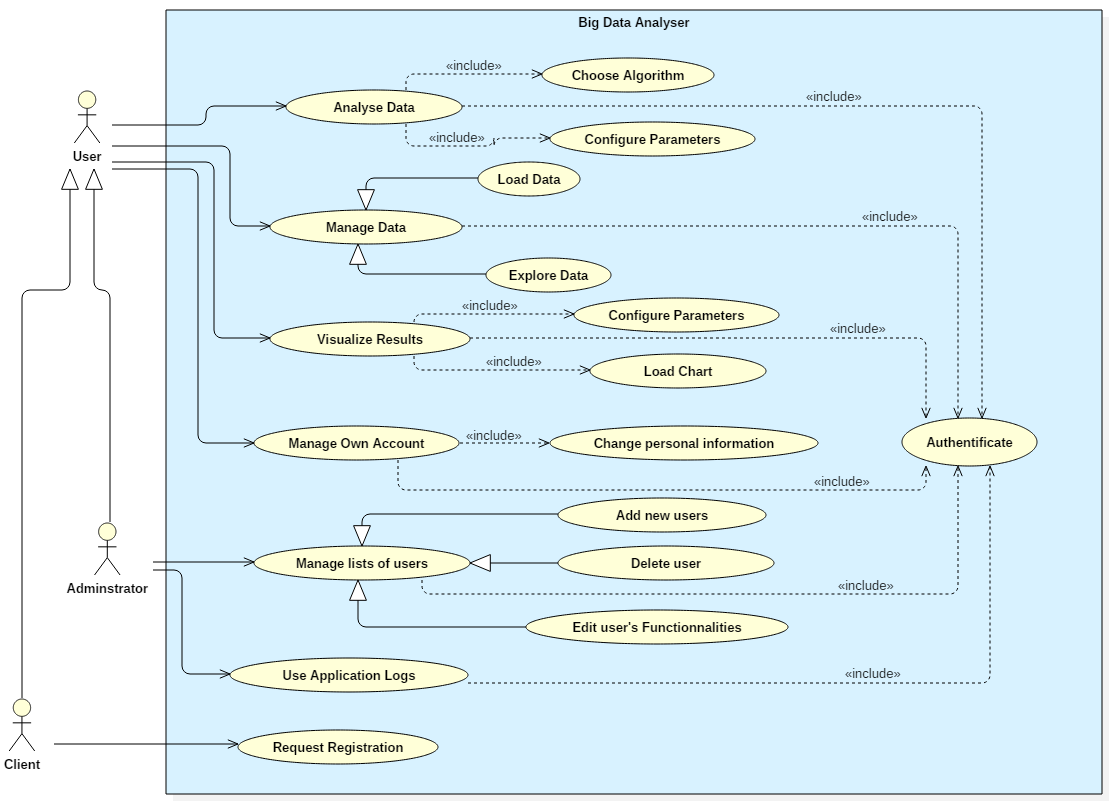
\includegraphics[width=17cm,height=16.3cm]{chapter3/userrusecase.png}
\end{center}
\caption{General Use Case}
\label{user}
\end{figure}

\begin{table}[H]
\caption{Use Cases Description}
\begin{center}
\begin{tabularx}{17cm}{|p{3.5cm}|X|X|}

\hline
	\textbf{Actor} & \textbf{Use Case} & \textbf{Description} \\ \hline
    \multirow{4}{*}{User}&Analyse  Data&Analyse data is the first main feature that should be provided. \newline A user should choose as a first step which algorithm to run. Then as a second step, the user should configure algorithm parameters before running it. \newline This use case must be preceded by an authentication. \\ \cline{2-3}
    &Manage Data&Mange large scale of data is the second main feature that should be provided. User should be enabled to load data and explore its emplacement. \newline This use case must be preceded by an authentication.\\ \cline{2-3}
    &Visualize Results&Visualize results is also a main feature of the application. Result are sort of graphs and charts. Therefore, user should configure parameters (e.g. choosing axes) and then load chart. \newline This use case must be preceded by an authentication.\\ \cline{2-3}
    &Manage Account&The application must enable users to manage their own information in their accounts (e.g. password, user name ..). \newline This use case must be preceded by an authentication. \\ \hline
    
     
    \multirow{2}{*}{Administrator}&Manage list of users&The Administrator has exclusively the right to confirm new users’ right to access to their accounts after verifying their identity. \newline As being a critical use case, this operation must be preceded by authentication.\\ \cline{2-3}
    &Use Application Logs&Each operation processed must be logged in a way that enables the administrator to control application operations. \newline This use case is very important in order to register traceability of the processed operations which make reporting issues easier and more efficient. \newline This use case must be preceded by an authentication. \\ \hline
    
    
    Client&Request Registration&As a first step to interact with our application, a user should fill a form on which he describes his identity.\newline After this step, he waits for the administrator confirmation to access the application.\\
    \hline
    
\end{tabularx}
\end{center}
\label{description}
\end{table}


\subsection{Activity Diagram}
\subsubsection{Administrator Activity Diagram} 
The figure \ref{act1} shows an activity diagram that describes the flow of control relative to the \textbf{administrator}. It illustrates the main possible activities, actions and decisions made through interaction with the system.\\
  
When the administrator open the application on his web browser, he receives first the login page. He types his login name and password; if they (login + password) are correct, he will have access to the application. Otherwise, his request will be rejected and he will redirected again to the login page again. After getting the access to the application, the administrator will main menu. The provided options are \textbf{Manipulate Data}, \textbf{Choose the Manage List of users} and \textbf{Choose the Consult Application Log option}. If the user chooses the \textbf{Manage List of Users} option, he will be asked either to \textbf{Add new user}, \textbf{Delete existing User} or \textbf{Edit user features}.


\begin{figure}[H]
\begin{center}
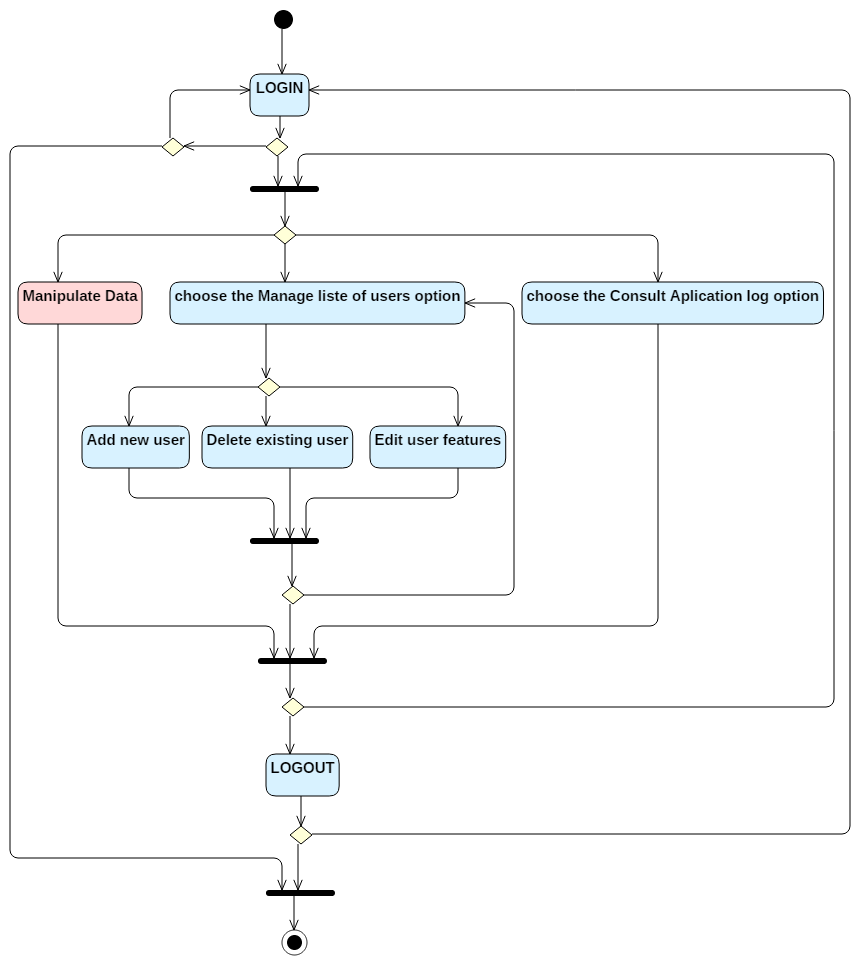
\includegraphics[width=17cm,height=16.7cm]{chapter3/administrator.png}
\end{center}
\caption{Administrator Activity Diagram}
\label{act1}
\end{figure}


\subsubsection{Client Activity Diagram}


The figure \ref{act2} shows an activity diagram that describes the flow of control relative to the \textbf{client}.\\

As a first step, a client should fill the registration form, providing his personal information. Filling this form is considered as a request to get access to the application. After this step, the client will wait for a confirmation from the administrator; if he get it (the confirmation), he will be able to access after. Otherwise, he will be rejected to fill a request again or quit the system.\\

Getting the confirmation will give the client the ability to login the system, manipulate his own data as much as he wants and then leave by logging out.  

\begin{figure}[H]
\begin{center}
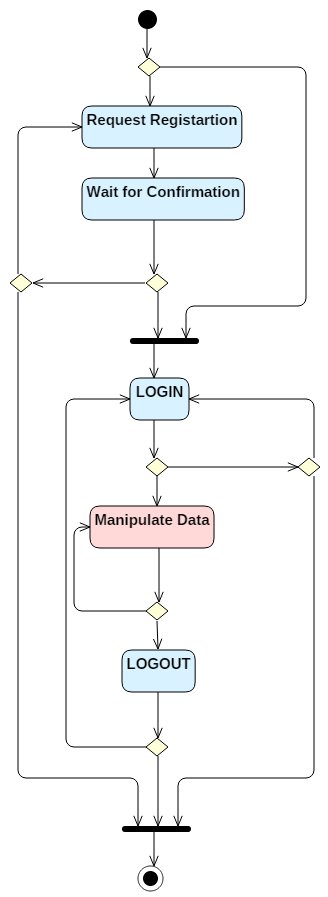
\includegraphics[width=7.5cm,height=17cm]{chapter3/client.png}
\end{center}
\caption{Client Activity Diagram}
\label{act2}
\end{figure}

\subsubsection{General User Activity Diagram}
The figure \ref{act3} shows a general activity diagram that describes the flow of control relative to the common operation for both actors which is: \textbf{Manipulate data}. When the user sits in front of his computer, open the application on his browser he receives, first, the authentication page. He types his login name and password. If it matches together (login + password), the user access to the application. Otherwise, he will redirected to the login page again. After getting the access the application, the user receives the main menu, from which he can choose either \textbf{Manage Data}, \textbf{Analyse Data} or \textbf{Visualize Data}. \\

 If the user chooses the \textbf{Manage Data} option, he will we asked to choose if he wants to load new data or to explore existing data through a file manager. If the user chooses the \textbf{Analyse Data} option, then he is asked which is the appropriate algorithm to run on selected data, configure the algorithm parameters and process it by the end. If the user chooses the \textbf{Visualize Data} option, then he will be asked to fill the configuration form (select result to visualize, select axes …). This step will make loading charts possible. 

After all, the user will have the choice either to to logout from the application or to operate again one of the previously mentioned options.\\


\begin{figure}[H]
\begin{center}
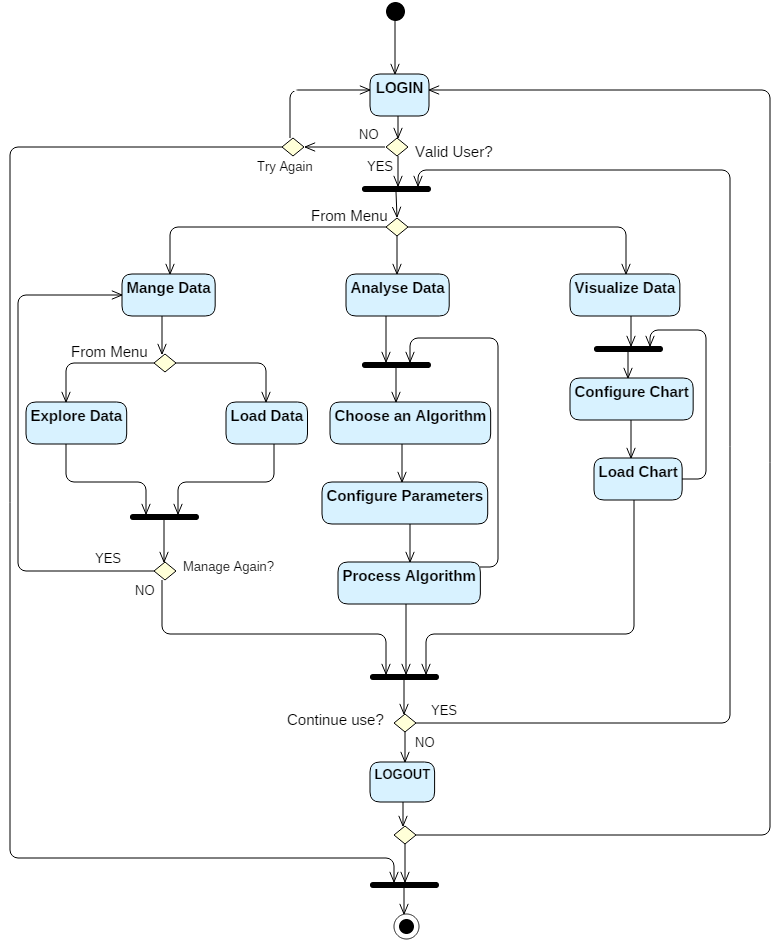
\includegraphics[width=17cm,height=15cm]{chapter3/activity.png}
\end{center}
\caption{General user Activity Diagram}
\label{act3}
\end{figure}




 
\section*{Conclusion}

In this chapter, we have presented the requirements and the needs of the system and its users. We have first identified the actors of our system and explicit the functional and non-functional requirements. Then, we have detailed these needs by specifying, in more details, the features expected through a detailed use case and activity diagram. Thus, we can begin the design phase, which will be the purpose of the next chapter.

\chapter{Design and Structure}
\label{Chapter4} 
Through results gathered from the previous chapter according analyzing and specifying the requirements of the project, we can now start the design step as it is a crucial and aim to undertake and prepare the ground for the implementation step. In this chapter, we will present our conceptual approach as well as arguments for this choice. Then we explain the detailed design.
\section{Global Design}


\subsection{Architectural Overview}
 
Figure \ref{phy} shows the physical architecture of the system. It includes the different material component that build our applications infrastructure.  
 ~\\
\begin{figure}[!ht]
\begin{center}
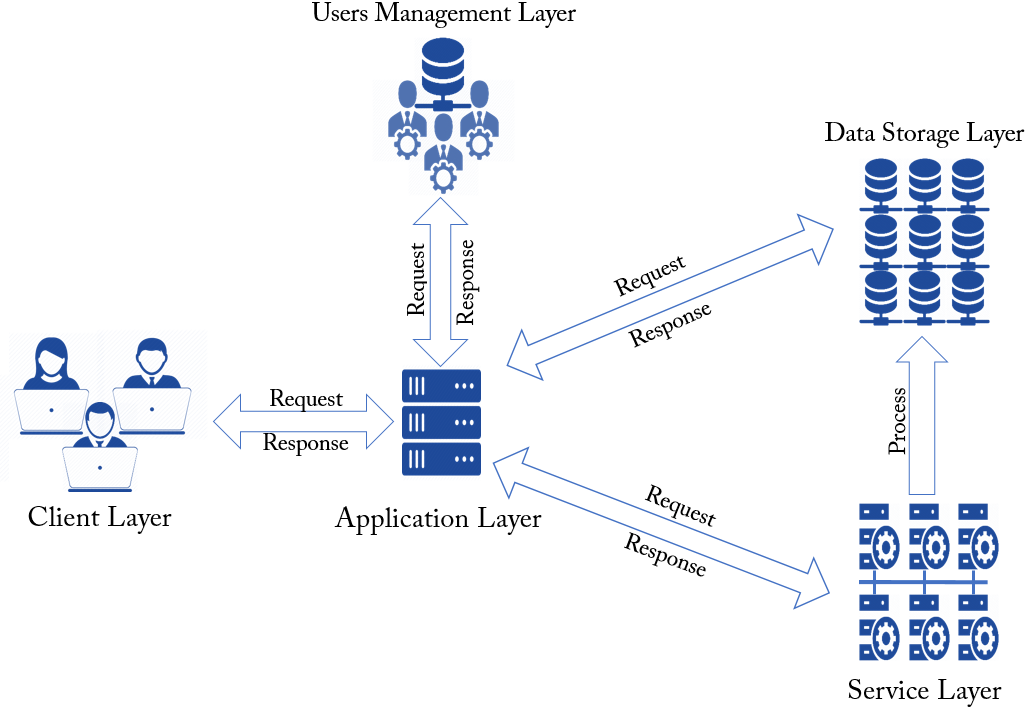
\includegraphics[width=17cm,height=10.2cm]{chapter4/fig1.png}
\end{center}
\caption{General Architecture of the System}
\label{phy}
\end{figure}
 
The software physical architecture is structured around 5 main layers. Every layer presents a different physical level of the application structure.
\begin{itemize}
\item \textbf{Client Layer:} is a display level of the application, includes the web view in the users browser.\\ 
\item \textbf{Application Layer:} is the web server, the module that executes the different component of our application core.\\
\item \textbf{Users Management Layer:} is data base server that contains the application users information, which make it possible for the application layer to manage users and their roles.\\
\item \textbf{Service Layer:} is the layer where the Spark core executes. It composed from a master cluster and many worker nodes dispersed in different clusters.\\
\item \textbf{Data Storage Layer:} is the layer where files are managed through Hadoop Distributed File System. This layer is composed from many clusters, each cluster is composed from many servers.\\
\end{itemize}
\subsection{Software Architecture}

Figure \ref{package} shows the software internal architecture. This architecture is illustrated through a package diagram.\\

\begin{figure}[!ht]
\begin{center}
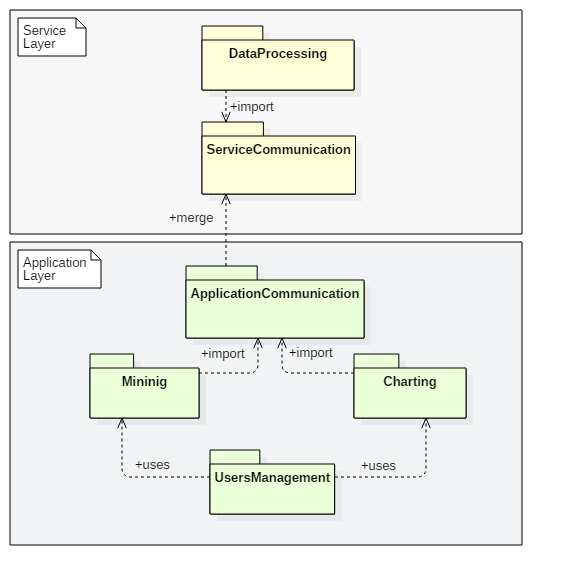
\includegraphics[width=15cm,height=10cm]{chapter4/package.png}
\end{center}
\caption{Packages Diagram}
\label{package}
\end{figure}

\begin{itemize}
\item \textbf{Service Layer:}\\
\begin{itemize}
\item \textbf{DataProcessing:} Contains Python classes that are supposed to execute Spark core. This package is a processing \\
\item \textbf{ServiceCommunication:} In this package we find all component needed to maintain communication between the service layer and the application layer through sockets queries.\\
\end{itemize}

\item \textbf{Application Layer:}\\
\begin{itemize}
\item \textbf{ApplicationCommunication:} is the application layer image for the ServerCommunication package. It communicates with the service layer through sockets queries.\\
\item \textbf{Mining:} is the package that gathers the different models of the used algorithms. This algorithm does not really execute the algorithm but it set the algorithm parameters in order to send it through sockets queries to the service layer that will be responsible to execute the desired algorithm.\\
\item \textbf{Charting:} For every algorithm model, there is a charting model which will present a personalized way the execution algorithm results.\\
\item \textbf{UserManagement:} is the layer that covers all model of user management such login, logout and roles given for each type of users.\\
\end{itemize}
\end{itemize}




\section{Detailed Design}
\subsection{Class Diagram}
Figure \ref{class} shows the class diagram of our proposed solution. Every class is presented on its containing package.\\

\begin{itemize}
\item \textbf{Service Layer:}\\
\begin{itemize}
\item \textbf{Kmeans:} Kmeans class is the controller class that executes the kmeans algorithm in Saprk core. its parameters are set through the received data from the application layer.\\
\item \textbf{Pca:} PCA class is the controller class that executes the PCA algorithm in Saprk core. its parameters are set through the received data from the application layer.\\
\item \textbf{DecisionTree:} DecisionTree class is the controller class that executes the decision Tree algorithm in Saprk core. its parameters are set through the received data from the application layer.\\
\item \textbf{LinearRegression:} LinearRegression class is the controller class that executes the Linear Regression algorithm in Saprk core. its parameters are set through the received data from the application layer.\\
\item \textbf{SocketServer:} SocketServer is class in service layer that implements all needed methods to make the executing service in permanent communication with the application.\\
\end{itemize}

\item \textbf{Application Layer:}\\
\begin{itemize}
\item \textbf{SocketClient:} SocketClient is the image class for the SocketServer in service side. It implements all the needed methods to communicate those from the socket server side (service layer).\\
\item \textbf{Pca:} Pca class is a model that make the application user sets the algorithms parameters and launch its execution in the service side.\\
\item \textbf{Kmeans:} Kmeans class is a model that make the application user sets the algorithms parameters and launch its execution in the service side.\\
\item \textbf{DecisionTree:} DecisionTree class is a model that make the application user sets the algorithms parameters and launch its execution in the service side.\\
\item \textbf{LinearRegression:} LinearRegression class is a model that make the application user sets the algorithms parameters and launch its execution in the service side.\\
\item \textbf{PcaChart:} PcaChart is the controller of the pca result chart load.\\
\item \textbf{KmeansChart:} KmeansChart is the controller of the pca result chart load.\\
\item \textbf{DecisionTreeChart:}  DecisionTreeChart is the controller of the pca result chart load.\\
\item \textbf{LinearRegressionChart:}  LinearRegressionChart is the controller of the pca result chart load.\\
\item \textbf{User:} User a class is a mother class that define all the common attributes and methods for any user type.\\
\item \textbf{Administrator:} Administrator class inherits all the methods and attributes from the User mother class. It define on type of users' roles by adding its own specific methods.\\
\item \textbf{Client:} Client is a specified class defined to represent a client type user. It inherits from the User mother class and implement its own specified methods.\\
\end{itemize}
\end{itemize} 


\begin{figure}[!ht]
\begin{center}
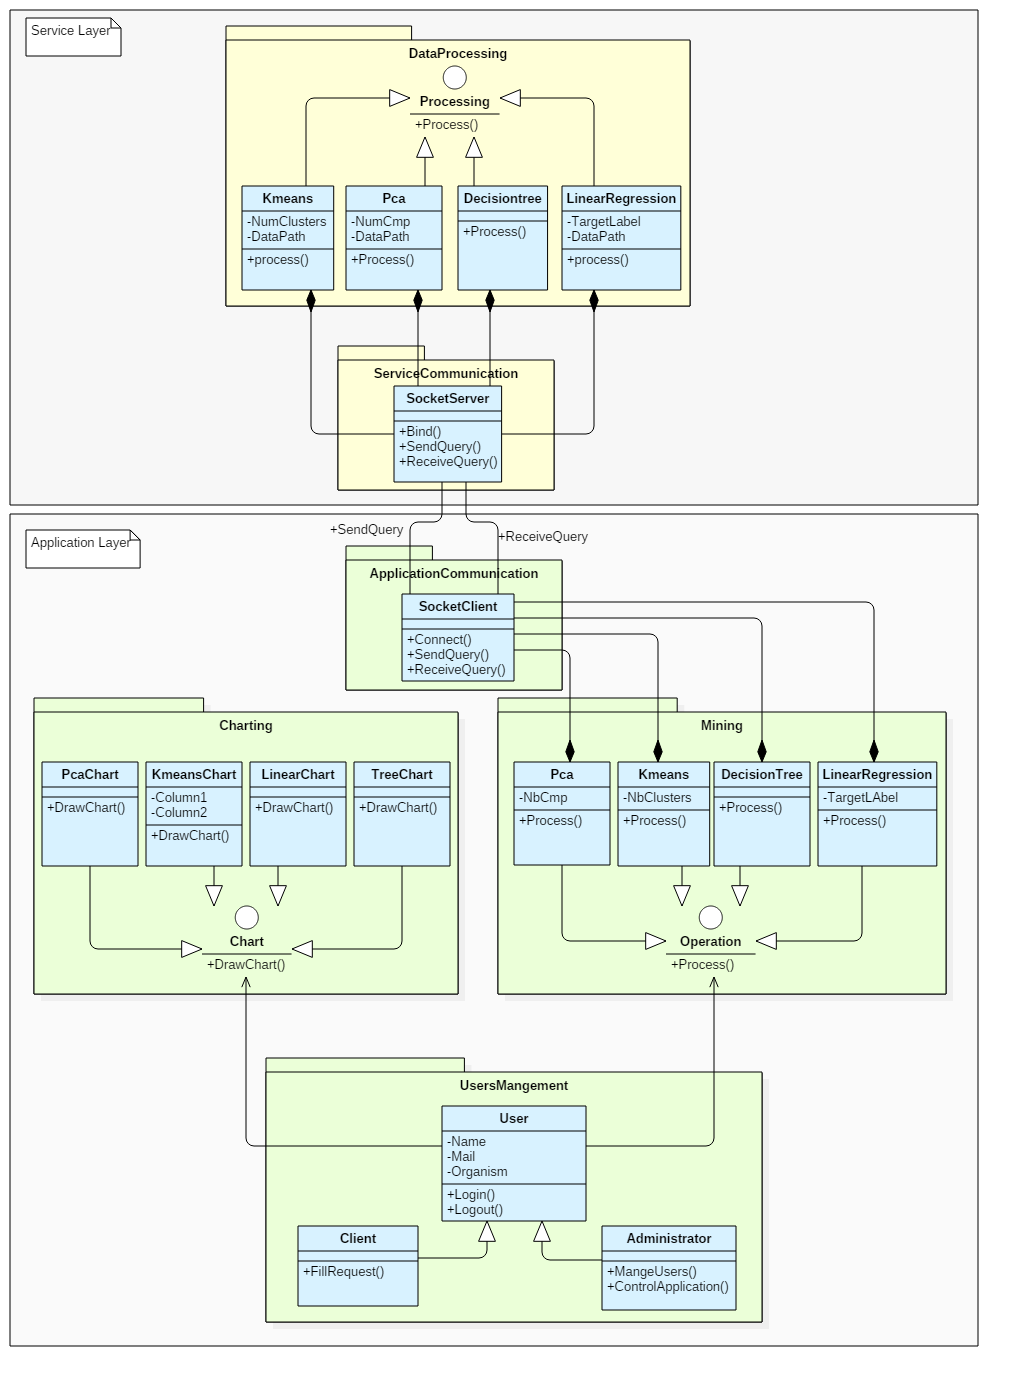
\includegraphics[width=17cm,height=23.5cm]{chapter4/class.png}
\end{center}
\caption{Class Diagram}
\label{class}
\end{figure}


\subsection{Sequences Diagrams}
\subsubsection{General Sequence Diagram}

Our system is mainly composed from 4 components; client side web application, a web server connected to a SQL data base to manage users accounts, a service server that runs operations on the data and many data storage servers. Figure \ref{seq0} shows the interaction between these different components when a user perform a single operation.\\

First the client types his login and password in the login form, the web server check in his data base and return either a failure notification ("wrong login and password") or a successful connection session to the client.\\

Throughout this session, the client can send a data load request to the web server, which will load data in data storage servers; if the operation is correctly done the user will be notified. In another step, the client will process an algorithm on a selected data. He will, then, select data and set the algorithm parameters. The web server will transfer this information to service server, which will run the algorithm and return a result file in a success case or an error notification otherwise. \\

The user can also load charts from the generated result files. He sets the chart parameter and the web server will take charge to draw the appropriate chart. \\

After finishing his job, the client can disconnect and the server will destroy the user session.\\

\newpage
\begin{figure}[!ht]
\begin{center}
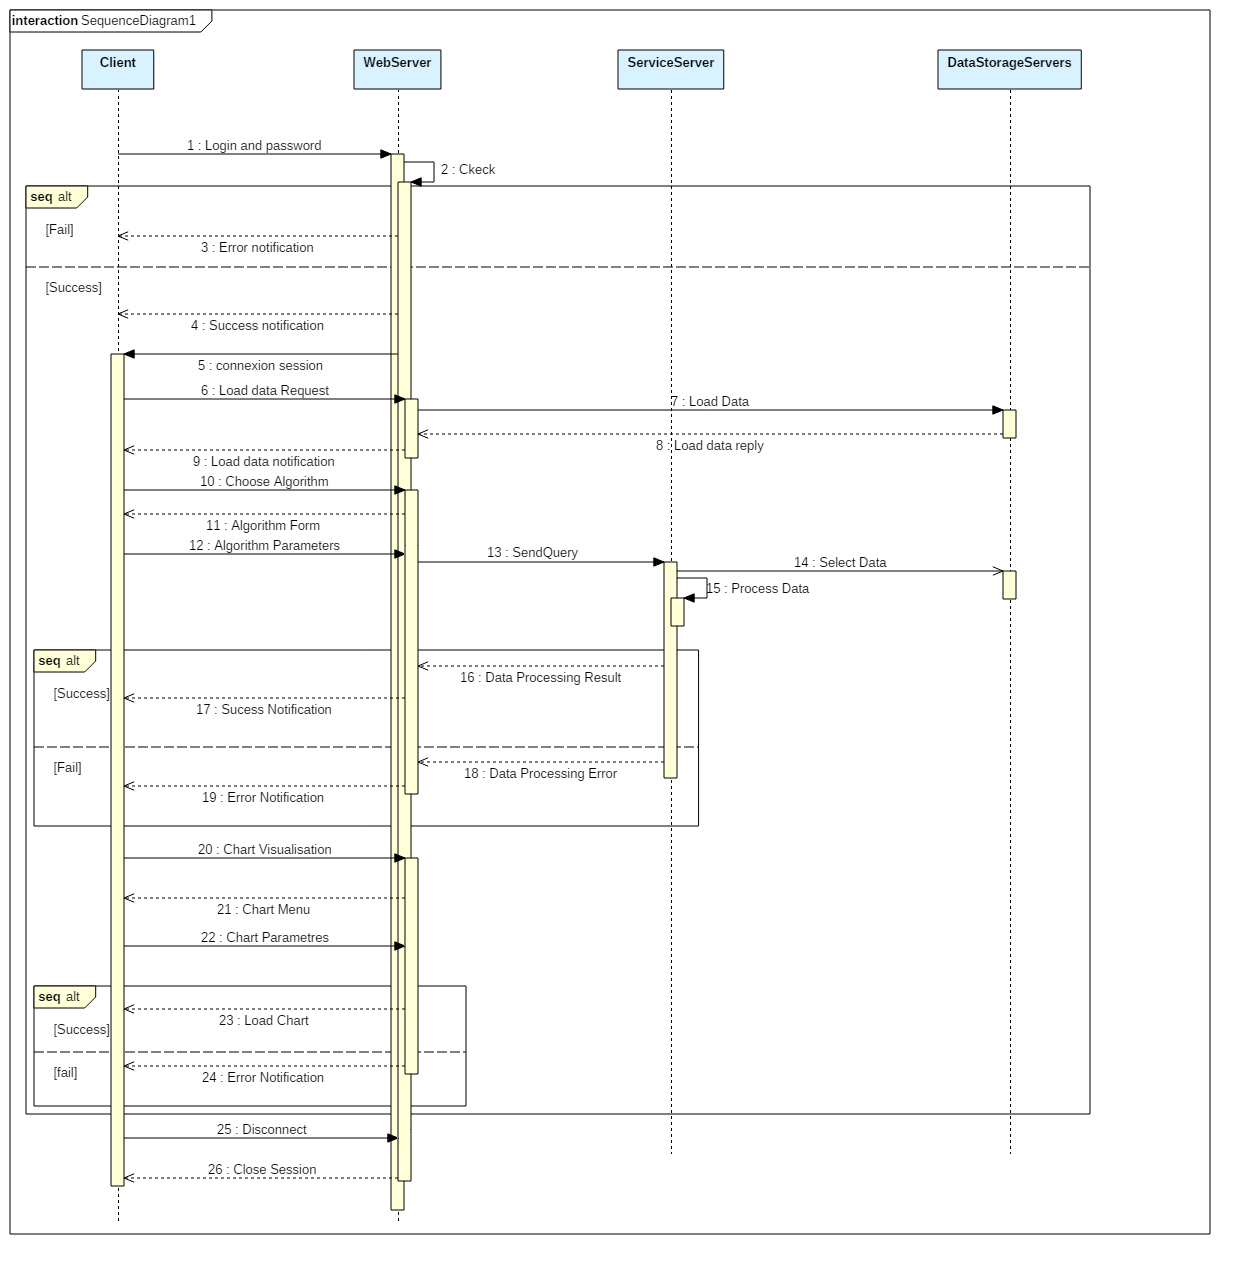
\includegraphics[width=17cm,height=24cm]{chapter4/sequence.png}
\end{center}
\caption{General Sequence Diagram}
\label{seq0}
\end{figure}
\subsubsection{Optimum Communication scenario}

Figure \ref{seq1} is a sequence diagram showing the optimum scenario of the connection established between the application server and the service server. This figure shows also the queries acknowledgement system that we have adopted to transfer the selected parameters from the user interface to the service server. First, the application ask for a TCP/IP connection. The service server establish the connection and create an appropriate thread for the actual operation. Then the application server send one parameter and wait for an acknowledgement  the send the next one. After sending all the needed parameters, the connection break down and the service server kill the operation thread. 

\begin{figure}[!ht]
\begin{center}
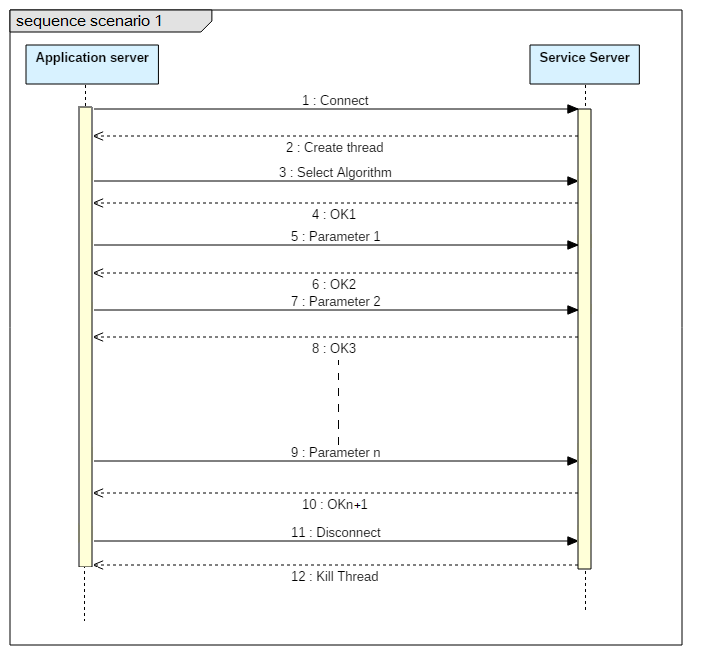
\includegraphics[width=12cm,height=13cm]{chapter4/SequenceDiagram1.png}
\end{center}
\caption{Optimum Communication scenario}
\label{seq1}
\end{figure}



\subsubsection{Lost Query Scenario}
Queries are the main way to make the application server and service server communicate. Queries are sent through TCP/IP sockets. In order to avoid server overload, if a query is lost the receiver will not wait for it infinitely. After exceeding a predefined timeout, the application layer will sent a query to disconnect from the service and then kill the attached service thread.\\

Figure \ref{seq2} describes this previously mentioned scenario.

\begin{figure}[!ht]
\begin{center}
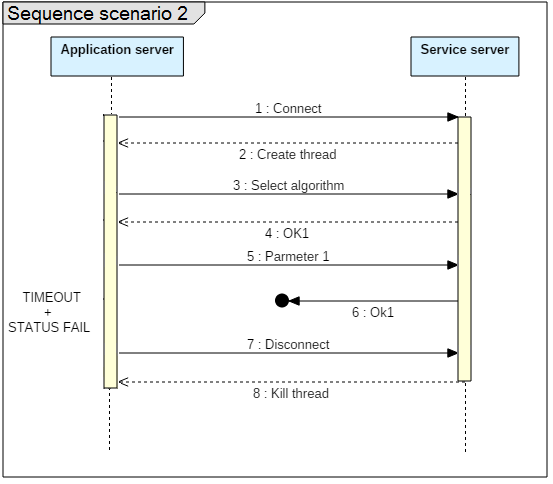
\includegraphics[width=9.3cm,height=8cm]{chapter4/SequenceDiagram2.png}
\end{center}
\caption{Lost Query Scenario}
\label{seq2}
\end{figure}




\subsubsection{Multi-Thread Communication Query Scenario}
In Order to grantee a multi-users application, we have adopted a multi-thread solution.  For every operation running in the service, we create a thread. As we are using a socket solution to send communication queries between the application server and the service server, there is a threat that a query sent from one thread disturb another one. In order to avoid the risk of disturbing the application, every sent or received query should be preceded by a user id in order to identify every query to whom user's thread belongs. If a thread receive a query that does not mind him, it will reject it and then inform the application server to send a query again. For every query received, the service thread make the same job, until it receive the correct query or reaches a maximum number of iterations; if it overcome it, it will reject the whole operation and kill the thread in order to avoid server overload and sudden shutdown.\\

Figure \ref{seq3} describes this previously mentioned scenario.  

\begin{figure}[!ht]
\begin{center}
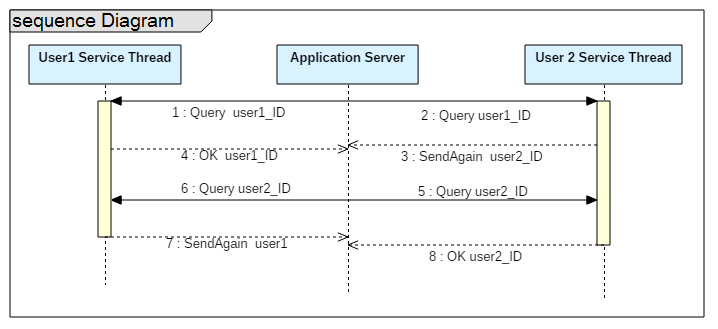
\includegraphics[width=11.5cm,height=7.5cm]{chapter4/SequenceDiagram3.png}
\end{center}
\caption{Multi-Thread Communication Query Scenario}
\label{seq3}
\end{figure}


\section*{Conclusion}

This chapter set the main guidelines on how we expect our solution to be. We started by giving an overview of our solution along with its physical architecture. Then, we provided various diagrams such as package, class and sequence diagrams to give more details on our solution's structure and interaction between its different elements. Since we agreed on the design of our solution, the next chapter will focus on the implementation
and the results we have reached.
\chapter{Implementation and Results}
\label{Chapter5} 


This chapter allows us to present the achieved work. We begin by listing the technologies and the software environment used throughout the project life cycle. After that, we present an overview of the achieved results and screenshots from different interfaces of our application. We end up this chapter with showing the flowed time-line during our project. 



\section{Implementation Environment}
\subsection{Hardware Tools}
To achieve this work we used a personal computer with the following characteristics:\\	

{\bf Workstation :}\\
Band: Laptop HP Probook 450 g3\\
Processor: Intel Core i7 CPU\\
Memory: 8,00GO of RAM\\
Operating system: Windows 10.


\subsection{Software Tools}

To achieve this work, we used  the software mentioned in the table \ref{sf}. More details in appendix A.
\begin{table}[!h]
\caption{Software Environment Characteristics}
\begin{center}
\begin{tabularx}{17cm}{ |p{4cm}|X|X| } 
 \hline
 \textbf{Tool} & \textbf{Category} & \textbf{Usage} \\ \hline
 Visual Studio 2012 Ultimate & Integrated Development Environment (IDE) & Developing the web controls.\\ \hline
Microsoft SQL Server & Database management system & Manage user information and users' accounts\\ \hline
Spyder & Integrated Development Environment (IDE) & Developing the service controllers.\\ \hline
Anaconda & Anaconda is a freemium open source distribution of the Python programming languages & Build the service.\\ \hline
Microsoft Project & Project Management Software & Developing plans and tracking progress. \\ \hline
\end{tabularx}
\end{center}
\label{sf}
\end{table}
\subsection{Technological Choices}
The table \ref{ut} shows the list of the used technologies. More details in appendix A.
\begin{table}[!h]
\caption{Used Technologies}
\begin{center}
\begin{tabularx}{17cm}{ |p{3cm}|X| } 
 \hline
 \textbf{Technology} & \textbf{Usage}  \\ \hline
 
C\# & The main programming language used for the code behind web pages.\\ \hline
ASP.Net & The used framework for developing the web controls. \\ \hline
DevExpress & The used library to design charts.\\ \hline
Python & The used programming language for implementing the service.\\ \hline
Apache Spark & Framework for processing data on parallel execution\\ \hline
HDFS & Distributed file system to store big data \\ \hline
Bootstrap & Framework for web design. \\ \hline
\end{tabularx}
\end{center}
\label{ut}
\end{table}
\section{Results}
\subsection{Execution Results}
\subsubsection{Behavior with Regard to the Number of Values}

The following charts show our solution performance according execution time and memory usage compared with result got from processing PCA algorithm on the same data using "KnowledgeNet Analytics" (Integration Object already used tool).
\begin{figure}[H]
\begin{center}
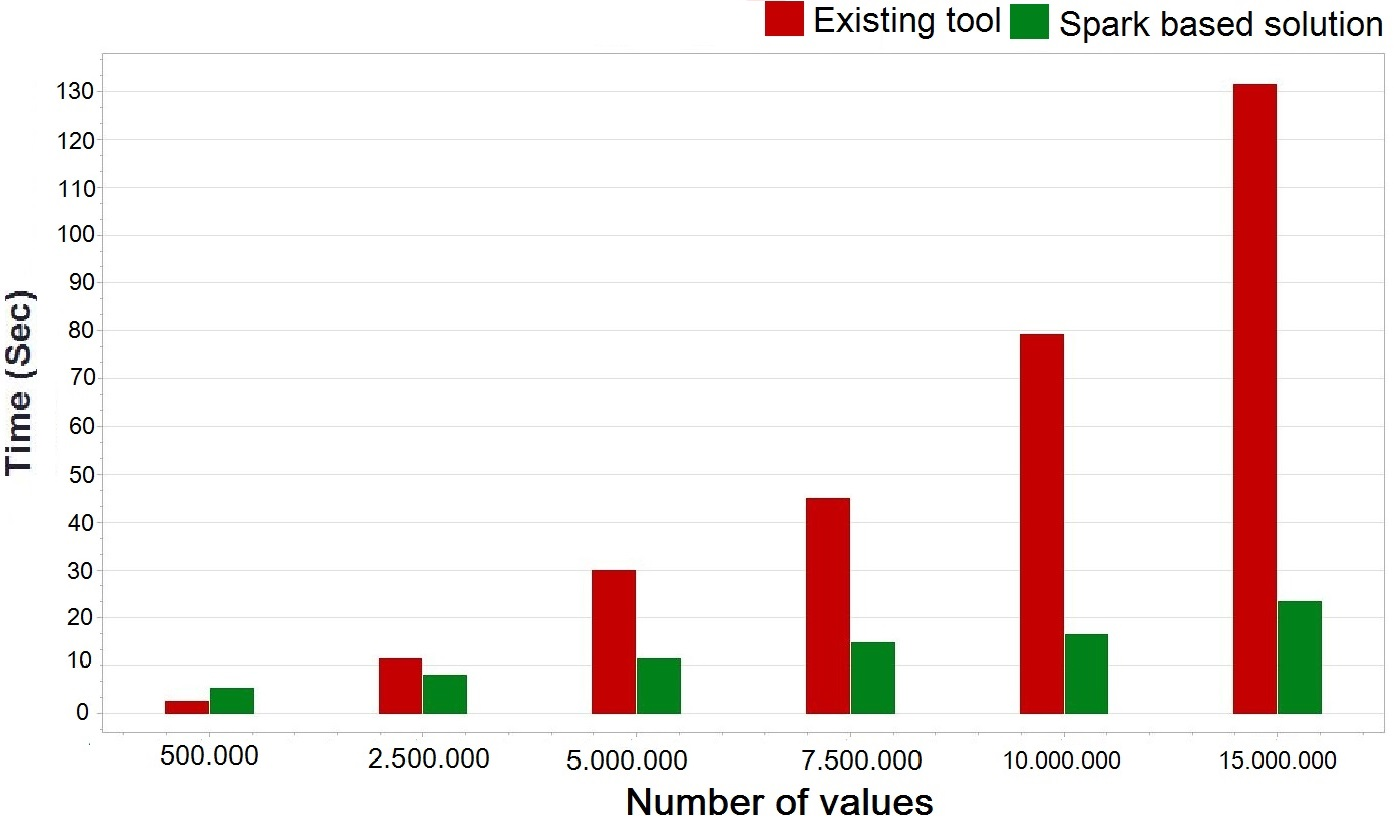
\includegraphics[width=15cm,height=8.5cm]{chapter5/1.JPG}
\end{center}
\caption{Execution Time test}
\label{teste1}
\end{figure}
Figure \ref{teste1} shows the difference between the already used tool and our implemented solution. For a data of 5.000.000 values KnowledgeNet Analytics processes PCA in 29.88 seconds while our solution process it in only 11.49 seconds (more than two times better). The more the data is big the more the difference is bigger. For a data of 15.000.000, KnowledgeNet Analytics takes 2min11s to process PCA while our solution takes 23.45 seconds (5 times better).
\begin{figure}[H]
\begin{center}
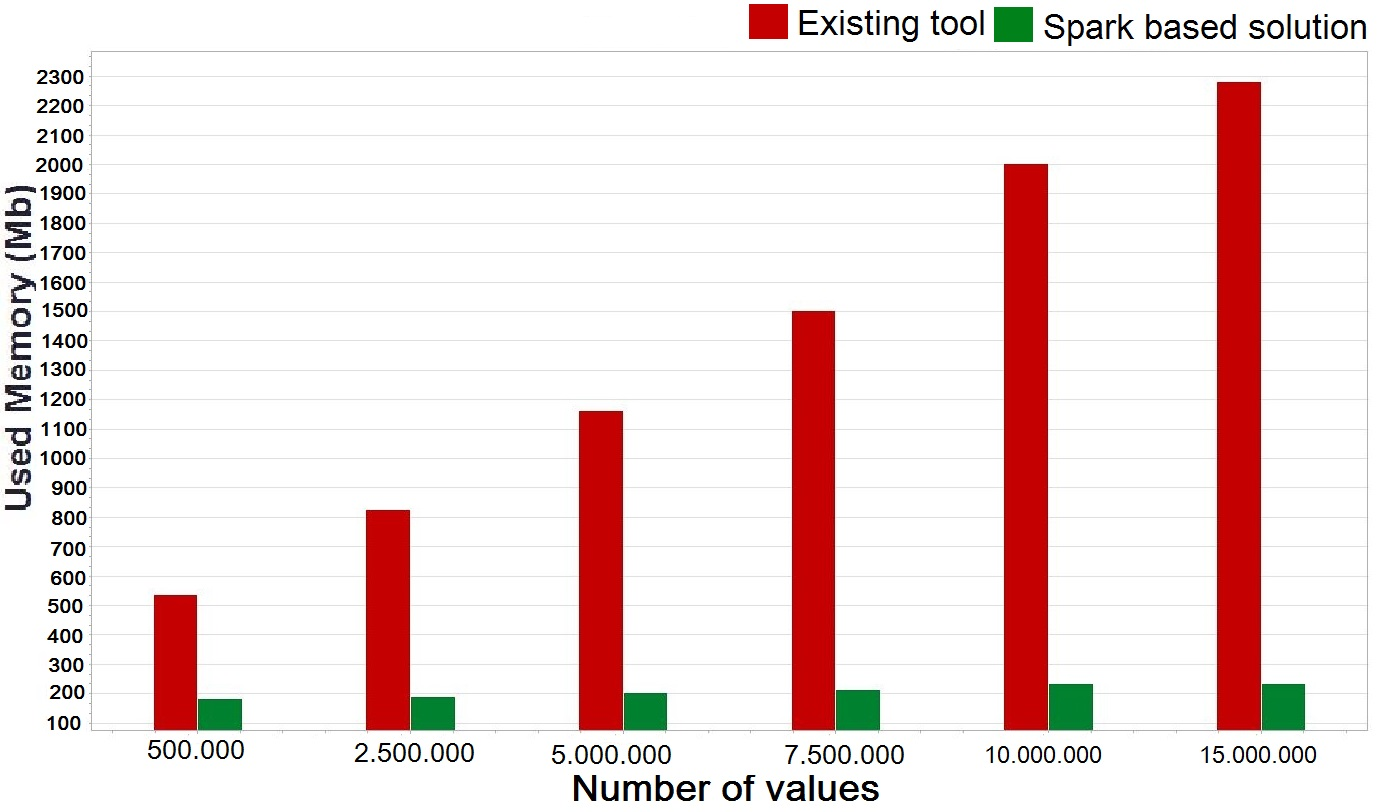
\includegraphics[width=15cm,height=8.5cm]{chapter5/2.JPG}
\end{center}
\caption{Memory Usage test}
\label{teste2}
\end{figure}
Our application doesn't perform execution time only, it also gives great performance in terms of memory usage. Figure \ref{teste2} shows how huge the difference is between KnowledgeNet Analytics and our solution.  For example, data of 5.000.000 values uses 1150 Mb of memory to process PCA algorithm. Our implemented solution takes only 233 Megabytes for more than 15.000.000 values.
\subsubsection{Behavior with Regard to the Number of Nodes}
Figure \ref{nodes} shows our solution behavior in term of run time vs. number of nodes. The used data is about 70 Megabyte of size.
\begin{figure}[H]
\begin{center}
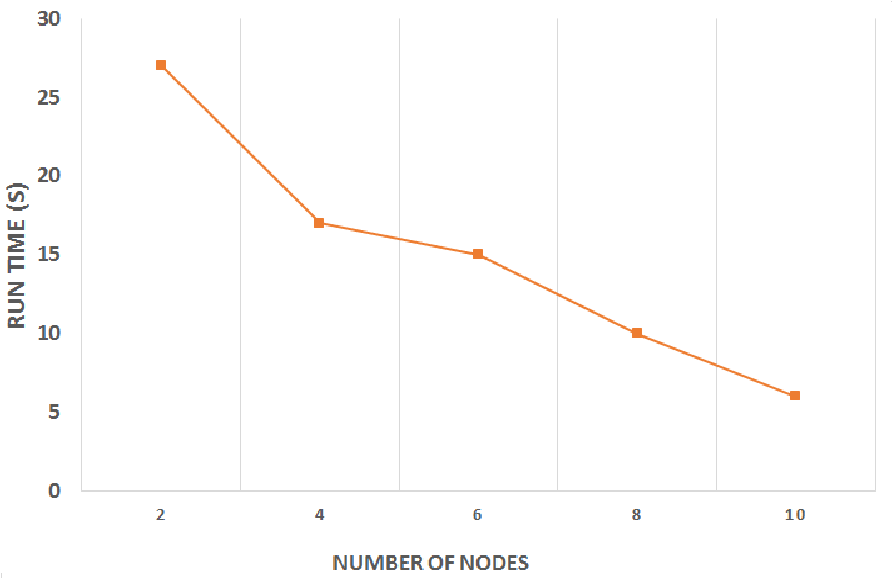
\includegraphics[width=13cm,height=7cm]{chapter5/nodes.png}
\end{center}
\caption{Time Performance Vs. Number of Nodes}
\label{nodes}
\end{figure}
\subsection{Illustrations from the Realization}

Figure \ref{explorer} shows the data explorer provided by our application. It provides all the needed functionalities to users to manage their own data. Thus they can create folders, upload csv files, move their files from one directory to another and many other features.\\

Figure \ref{chartpca} shows the chart loaded from the pca algorithm procced over data from a csv file. Results are shown after users configuration (axes and result file).\\

Figure \ref{chartkmeans} shows kmeans chart loaded. Clusters are represented by colours. Before loading the chart, the user have to fill the configuration form in order to suit the result to his needs.\\

Figure \ref{chartregression} shows linear regression chart. The result is represented with a scatter chart. A step of configuration precede the load of this chart.\\

~\\
~\\
~\\
~\\



\begin{figure}[H]
\begin{center}
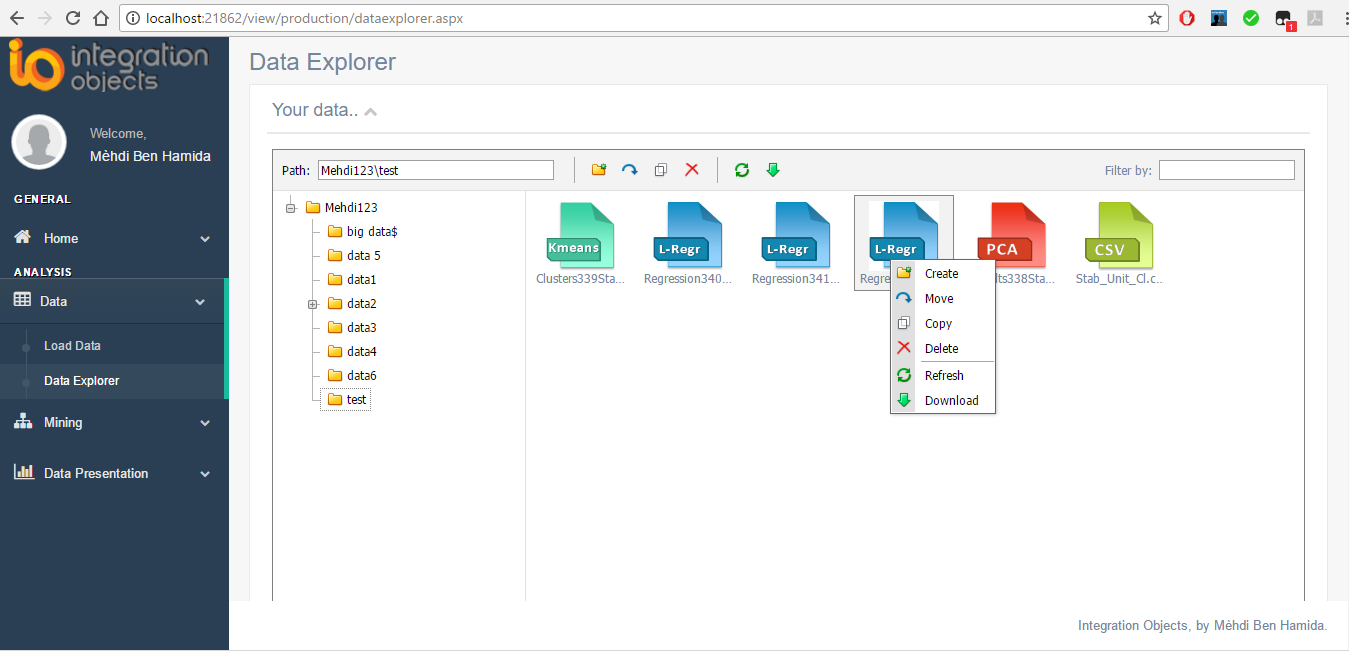
\includegraphics[width=17cm,height=10cm]{chapter5/dataexplorer.png}
\end{center}
\caption{Data File Manger}
\label{explorer}
\end{figure}

\begin{figure}[H]
\begin{center}
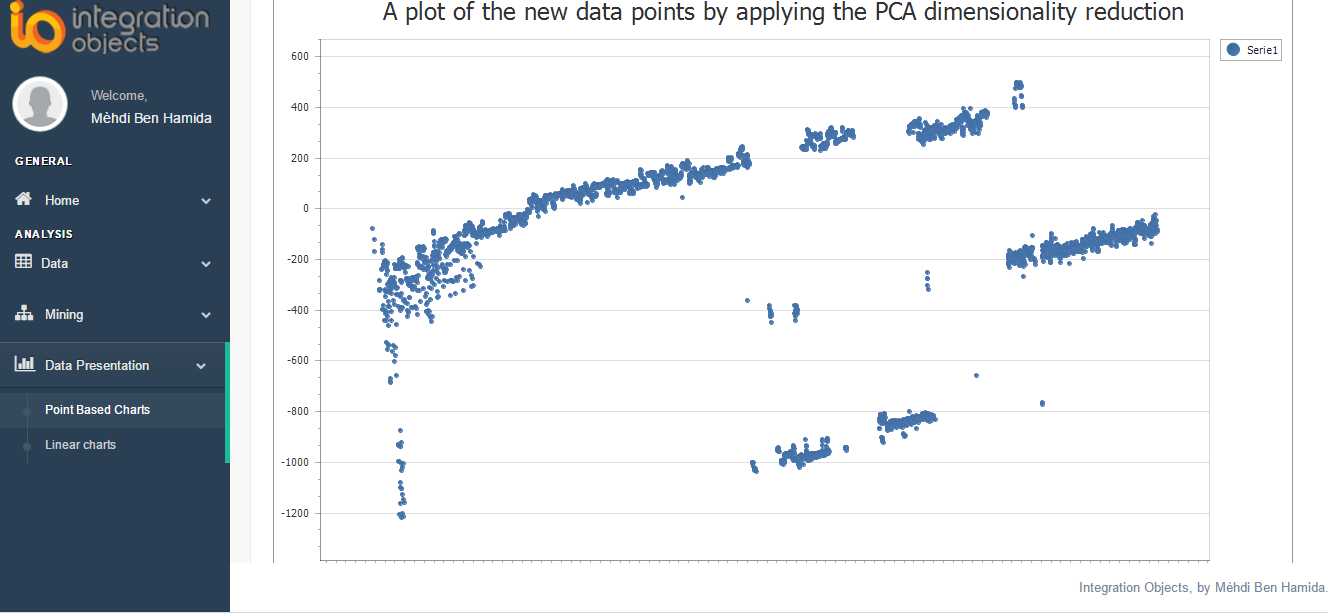
\includegraphics[width=17cm,height=10cm]{chapter5/pca.png}
\end{center}
\caption{PCA Results Chart}
\label{chartpca}
\end{figure}


\begin{figure}[H]
\begin{center}
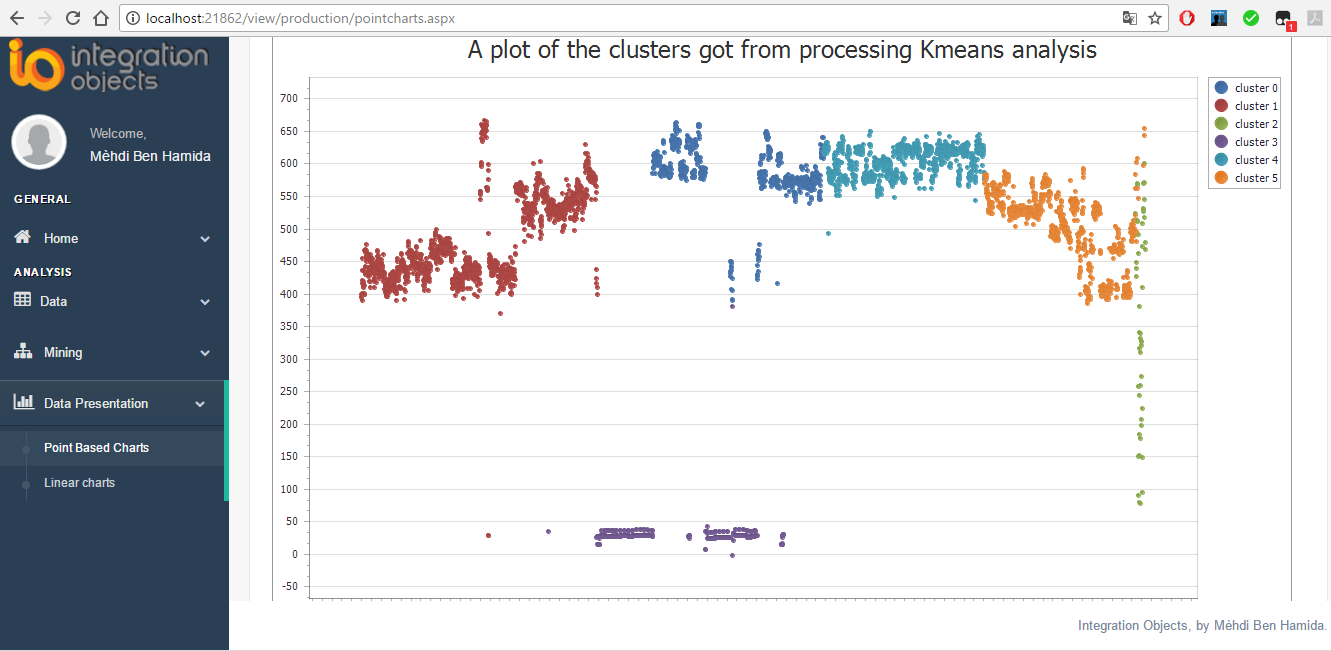
\includegraphics[width=17cm,height=10cm]{chapter5/kmeans.png}
\end{center}
\caption{Kmeans Results Chart}
\label{chartkmeans}
\end{figure}


\begin{figure}[H]
\begin{center}
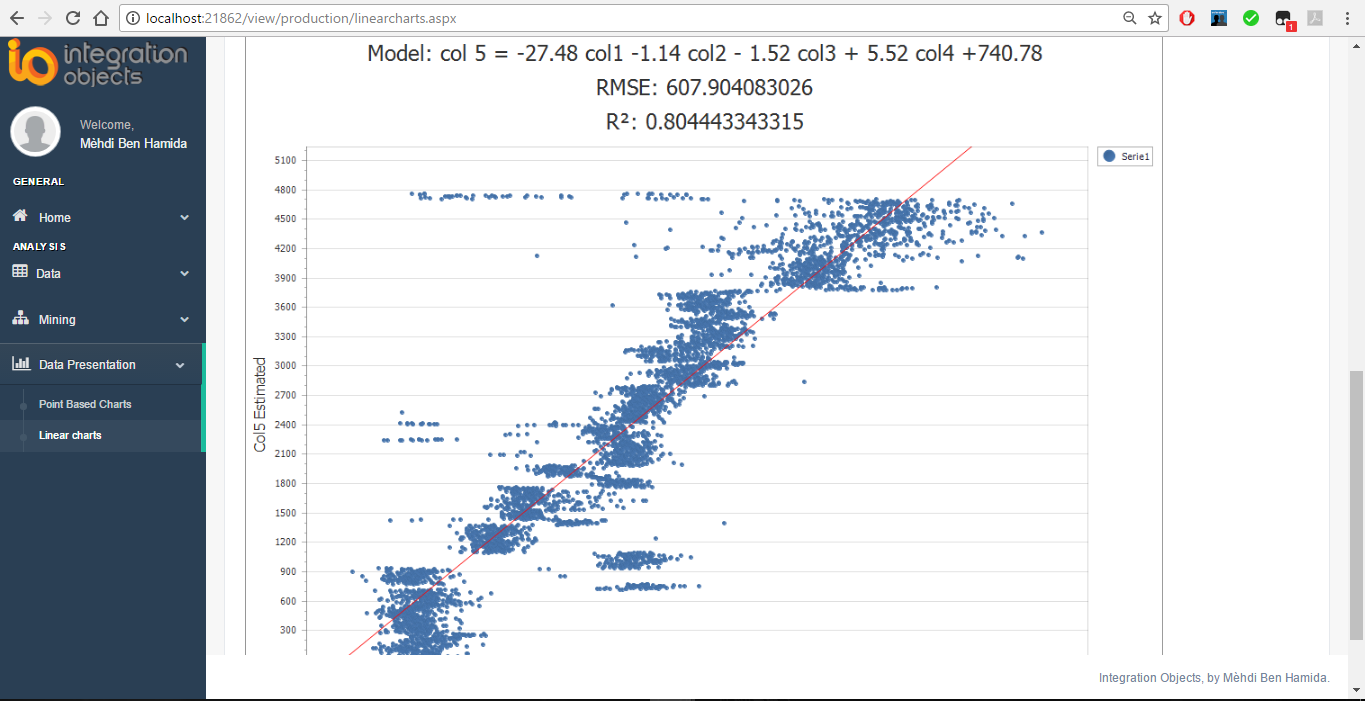
\includegraphics[width=17cm,height=11cm]{chapter5/linear.png}
\end{center}
\caption{Linear Regression Results Chart}
\label{chartregression}
\end{figure}
~\\
After a user launches an algorithm to be processed in the service server, a thread is created to be executed in a console application. Figure \ref{work} shows the background work in progress.\\

\begin{figure}[H]
\begin{center}
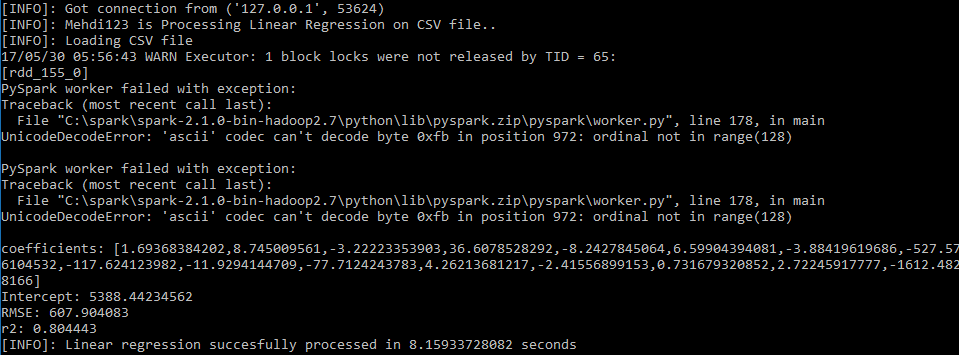
\includegraphics[width=17cm,height=7cm]{chapter5/work.png}
\end{center}
\caption{Background Service Server Execution}
\label{work}
\end{figure}
More achievement captures are represented in appendix \ref{achievement}.
\newpage


\section{Project Timeline}
The project timeline presented in the figure \ref{plan} describes how, we distributed the tasks achievement
during the sixteen weeks starting from February $1^{st}$, to May $31^{th}$.
\begin{figure}[H]
\begin{center}
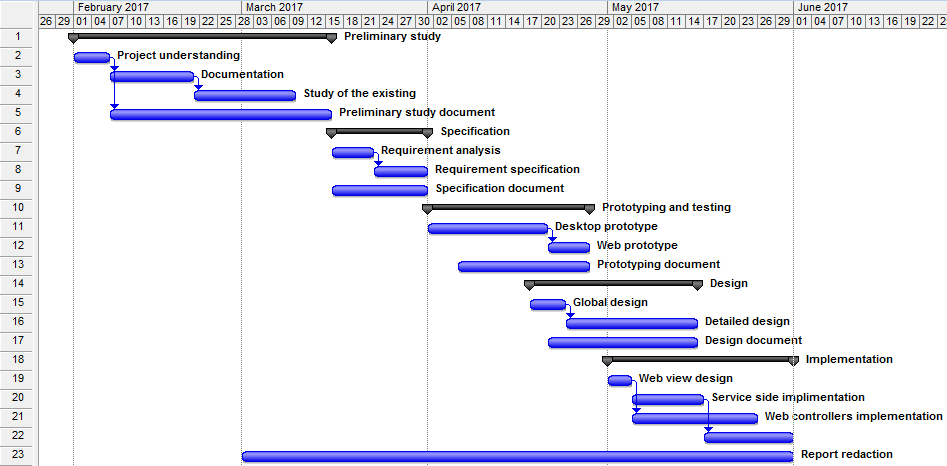
\includegraphics[width=17cm,height=9.7cm]{chapter5/plan.png}
\end{center}
\caption{Project Timeline}
\label{plan}
\end{figure}
\section*{Conclusion}
This final chapter described the implementation phase of our project. First, it presented the tools that we had used during the project life cycle. Then it presented some interfaces offered by our solution, in order to check the correspondence with the requirement specification.
\chapter*{Conclusion} 
\addcontentsline{toc}{chapter}{Conclusion}

As we are in the data era, data analysis has become one of the crucial computer sciences fields. Challenges beyond data analysis are growing more and more, and providing exploitable results from processing a large scale of data has become a priceless fortune for data owners.\\

The aim of this final graduation project is to design a suitable solution to process huge amount of data in order to run data mining algorithm without falling in the matter of slow data processing or out of memory issues, and to implement a graphical user interface that make it easy for costumers to visualize meaningful results.\\

Throughout this report, we have detailed the different phases of our project's life cycle starting with a preliminary study in which we defined some useful concepts then we have examined existent solution to our problem. Following, was the requirements specification where we have presented our application needs through functional and non-functional requirements. Then, we have focused on the design stage by elaborating class and sequence diagrams. Finally, we have proceeded to the implementation phase where we have exposed the achieved work.\\

Throughout this project, we faced various challenges related to the design of an advanced architecture and adapting it to big data manufacturing tools, in the search of the best possible performance. Merge from the desktop first prototype to a web based solution was also a challenge during this project, and it was made through separating executing components in our architecture.\\

For the next release, many extensions are expected to be added to our current solution. Indeed, we can add more data mining algorithms to our application and use the provided results to offer more expressive visualization for our application costumers. Nodes and clusters are also an important component of our system performance for either storage or processing data. Thus, improvements can cover this level also. 



%choix du style de la biblio
%\bibliographystyle{plain}
%inclusion de la biblio
\bibliographystyle{unsrt}
\bibliography{bibliographie}
\addcontentsline{toc}{chapter}{Bibliography}
\begin{appendix}
\chapter{Software \& Technologies}
In this appendix we will present the details of the software and the technologies used for achieving this
work.

\begin{itemize}
\item \textbf{Software environment:}
\begin{itemize}
\item \textbf{Microsoft Visual Studio:}\\
Microsoft Visual Studio is an integrated development environment (IDE) developed by Microsoft. It is
used for developing web sites, web services and in our case, web applications.
This software includes code editor, components for code completion, debugger and other features
offering a multitude of options for developers. This IDE supports different programming languages
such as C\#, HTML, JavaScript and many others.
\item \textbf{Microsoft SQL Server:}\\
Microsoft SQL Server is a relational database management system from Microsoft. It offers a set of programming extensions that add several features to standard SQL including row processing,
error handling and transaction control.
\item \textbf{Spyder:}\\
Spyder is an open source cross-platform integrated development environment (IDE) for scientific programming in the Python language. Spyder integrates NumPy, SciPy, Matplotlib and IPython, as well as other open source software. Spyder is extensible with plugins, includes support for interactive tools for data inspection and embeds Python-specific code quality assurance and introspection instruments. It is available cross-platform through Anaconda, on Windows with WinPython and Python(x,y).
\item \textbf{Anaconda:}\\
Anaconda is a freemium open source distribution of the Python and R programming languages for large-scale data processing, predictive analytics, and scientific computing, that aims to simplify package management and deployment. Package versions are managed by the package management system conda.
\item \textbf{Microsoft Project:}\\
Microsoft Project is a project management software developed by Microsoft. It helps plan, organize
and manage estimation, planning and scheduling. We used this software in order to keep the work
organized and respect the time lines for the project's different steps.
\newpage
\end{itemize}
\item \textbf{Technologies:}
\begin{itemize}
\item \textbf{C\# Programming Language:}\\
C\# is an object oriented programming language from Microsoft. It enables
developers to build secure and robust applications. It also permits to develop applications that run on the .Net framework.
\item \textbf{ASP.NET Framework:}\\
Asp.net is a free web framework used for developing and building
web applications using different languages such as HTML, CSS, JavaScript and many others. This web framework offers three different frameworks for creating web applications: ASP.NET Web Pages, ASP.NET Web Forms, ASP.NET MVC. All of the three frameworks mentioned above offers the
same facilities that are part of the core ASP.NET framework.
\item \textbf{DevExpress:}\\
DevExpress is a custom third party provider of .NET controls. They customize the .NET controls by making it more attractive and more flexible than inbuilt .NET controls.
\item \textbf{Python Programming Language:}\\
Python is a powerful high-level, object-oriented programming language. Python is an interpreted language, it has a design philosophy which emphasizes code readability through whitespace indentation, and a syntax which allows programmers to express concepts in few lines code. 
\item \textbf{Apache Spark Framework:}\\
Apache Spark is a fast and general engine for large-scale data processing. Spark powers a stack of libraries including SQL and DataFrames, MLlib for machine learning, GraphX, and spark Streaming. Spark extends its predecessors with in-memory processing. Its Resilient Distributed Dataset (RDD) abstraction enables developers to materialize any point in a processing pipeline into memory across the cluster, meaning that future steps that want to deal with the same data set need not recompute it or reload it from disk. Sparks runs on Hadoop, Mesos, standalone, or in the cloud.
\item \textbf{Hadoop Distributed File System (HDFS):}\\
HDFS is a distributed file system that provides high-performance access to data across Hadoop clusters. Like other Hadoop-related technologies, HDFS has become a key tool for managing pools of big data and supporting big data analytics applications.
\item \textbf{Bootstrap Framework:}\\
Bootstrap is an open-source Javascript framework developed by the team at Twitter. It is a combination of HTML, CSS, and Javascript code designed to help build user interface components.
\end{itemize}
\end{itemize}





\chapter{Achievements}
\label{achievement}
In this appendix we will show the different steps that should be followed to process an algorithm on a data.

~\\
~\\
~\\
~\\
~\\
~\\
~\\
~\\
\begin{itemize}
\item \textbf{Step 1:} Register\\

\begin{figure}[!ht]
\begin{center}
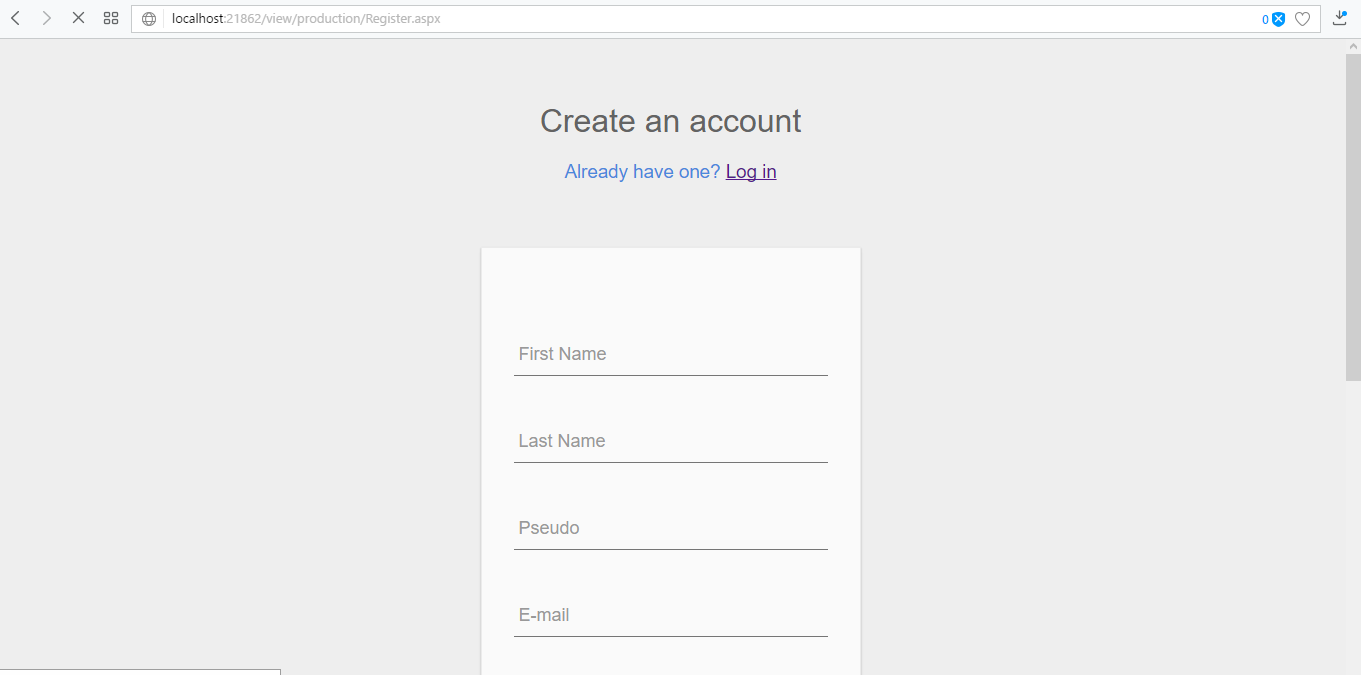
\includegraphics[width=17cm,height=10cm]{chapter5/register.png}
\end{center}
\caption{Register Page Capture}
\label{register}
\end{figure} 

\item \textbf{Step 2:} Login\\

\begin{figure}[!ht]
\begin{center}
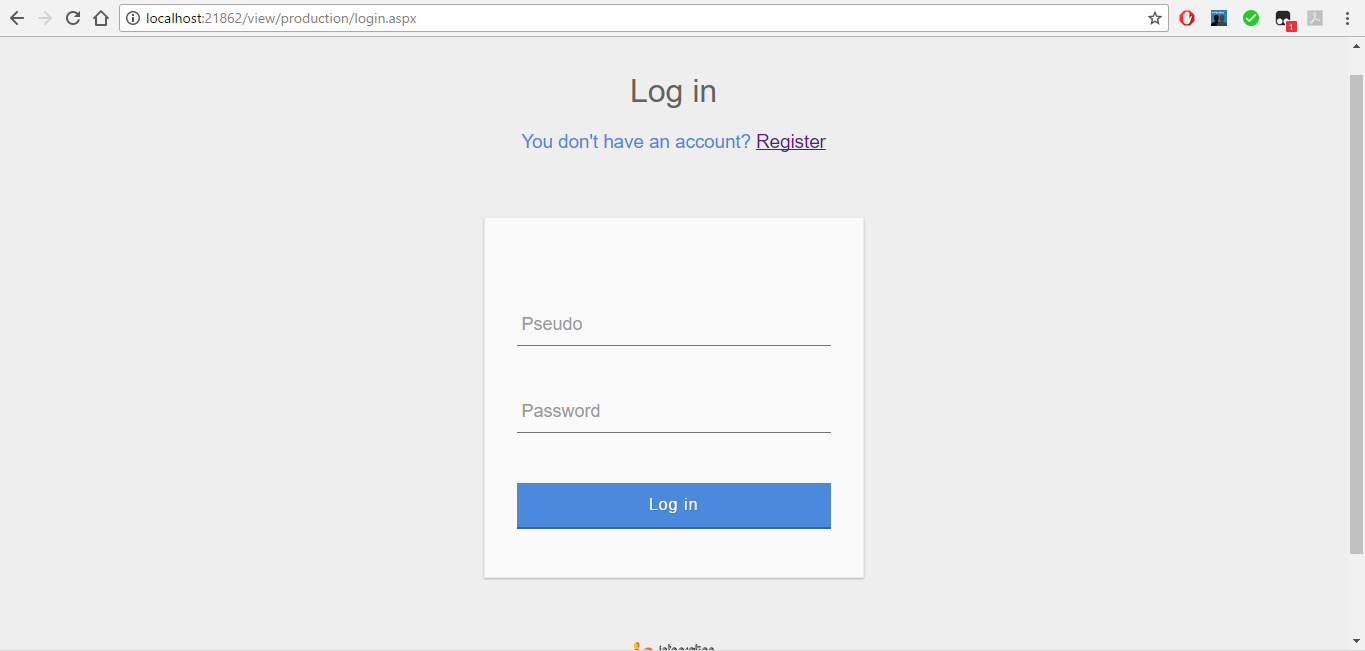
\includegraphics[width=17cm,height=10cm]{chapter5/login.png}
\end{center}
\caption{Login Page Capture}
\label{login}
\end{figure} 

\item \textbf{Step 3:} Load Data\\

\begin{figure}[!ht]
\begin{center}
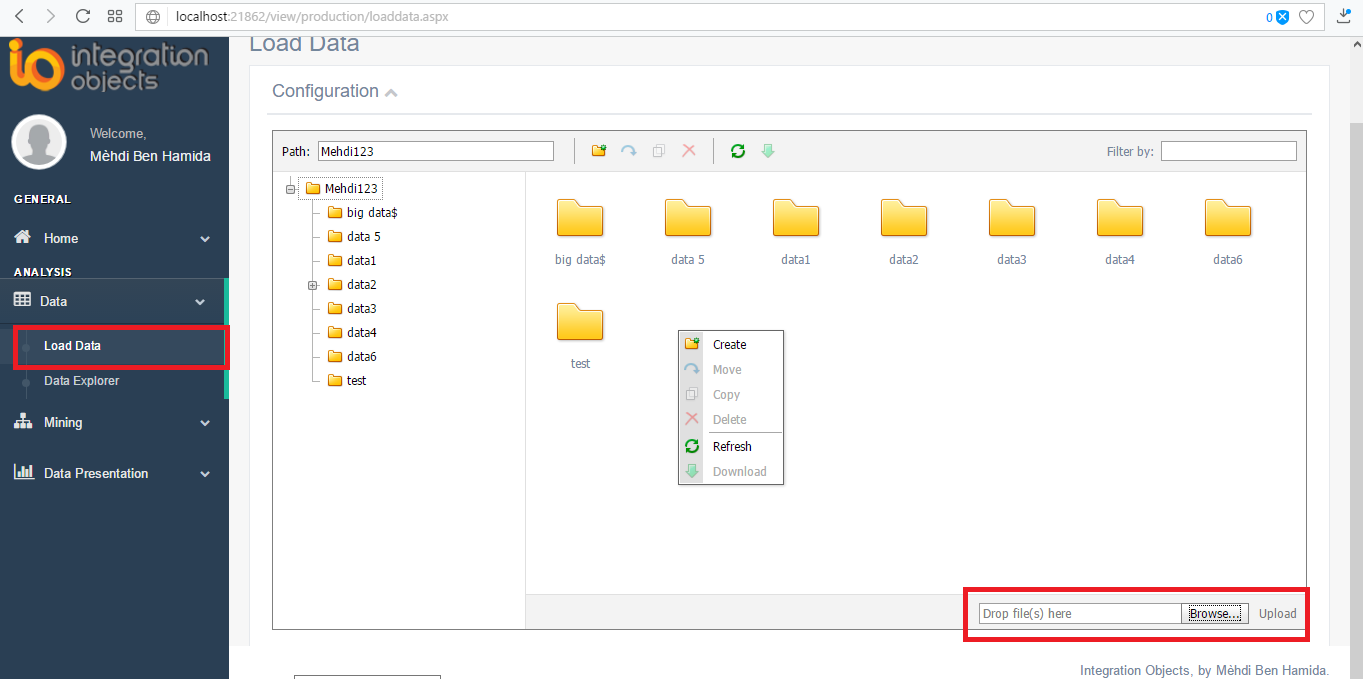
\includegraphics[width=17cm,height=10cm]{chapter5/load.png}
\end{center}
\caption{Load Page Capture}
\label{l}
\end{figure} 


\item \textbf{Step 4:} Select an algorithm\\

\begin{figure}[!ht]
\begin{center}
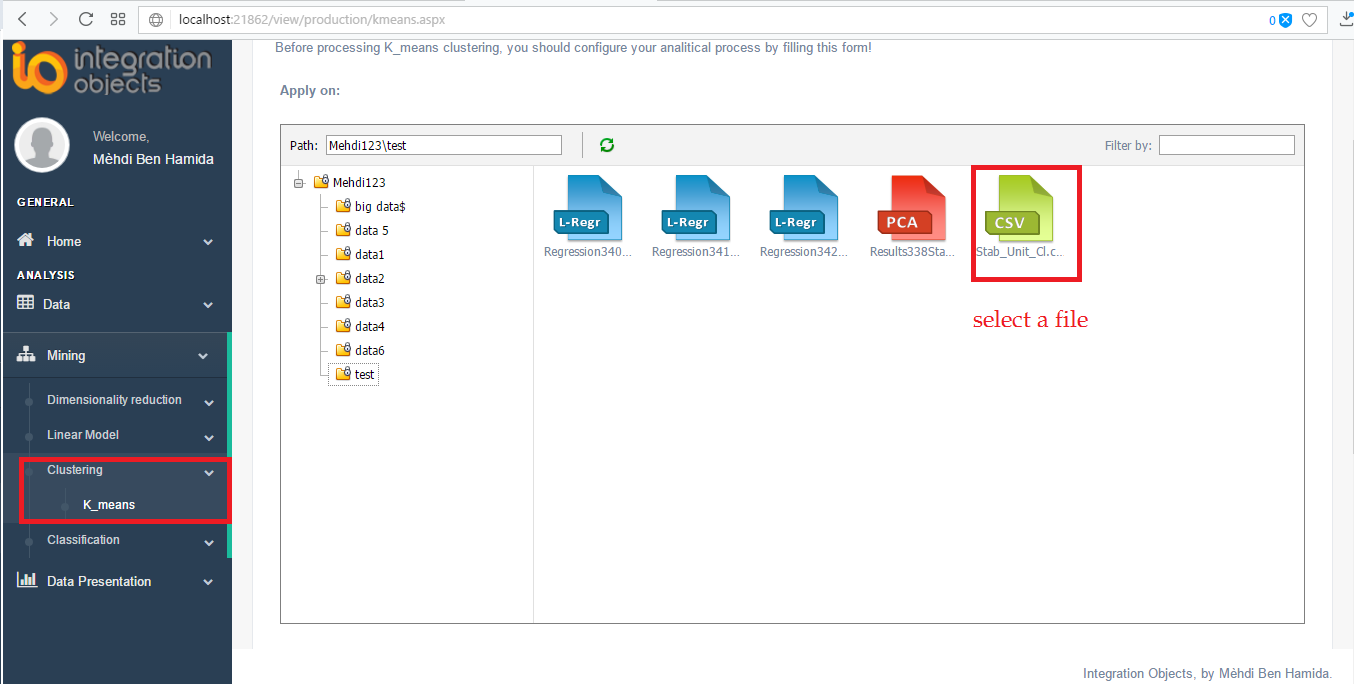
\includegraphics[width=17cm,height=10cm]{chapter5/k1.png}
\end{center}
\caption{Select Algorithm Page Capture}
\label{s}
\end{figure} 

\item \textbf{Step 5:} Set algorithm parameters\\

\begin{figure}[!ht]
\begin{center}
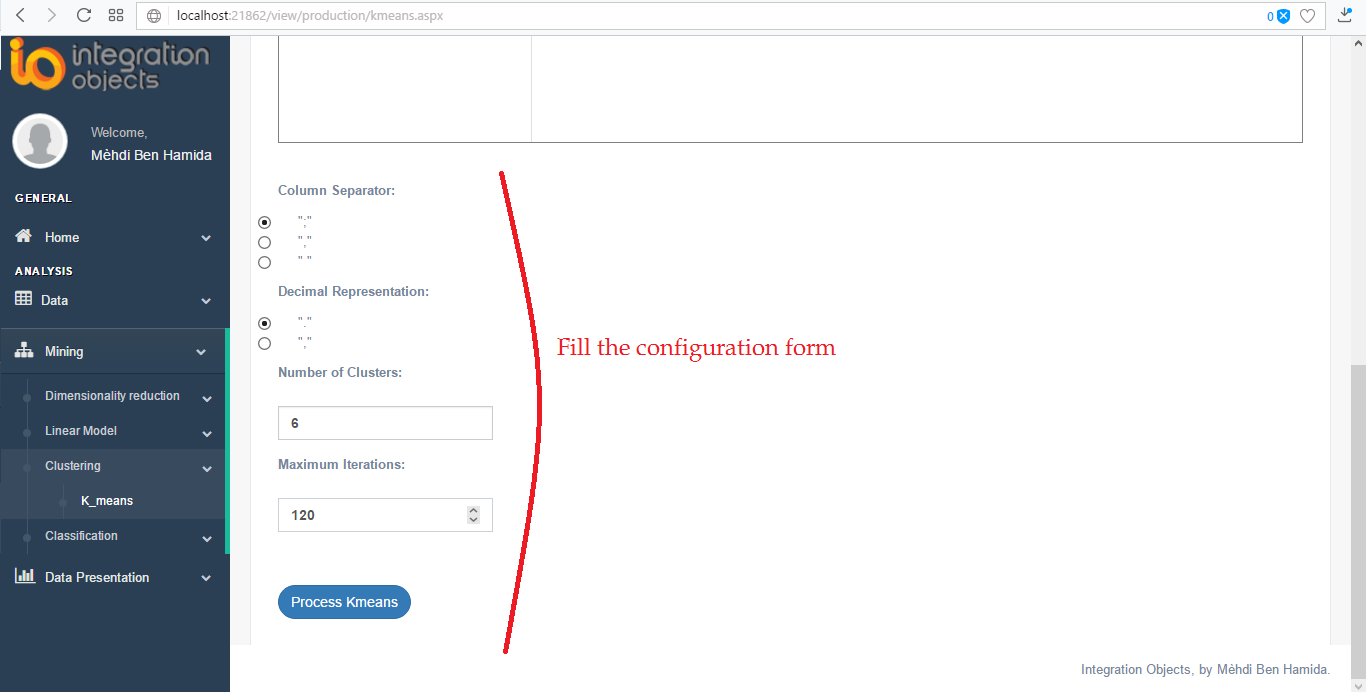
\includegraphics[width=17cm,height=10cm]{chapter5/k2.png}
\end{center}
\caption{Set Algorithm Parameters Page Capture}
\label{s2}
\end{figure} 

\item \textbf{Step 6:} Set chart parameters\\

\begin{figure}[!ht]
\begin{center}
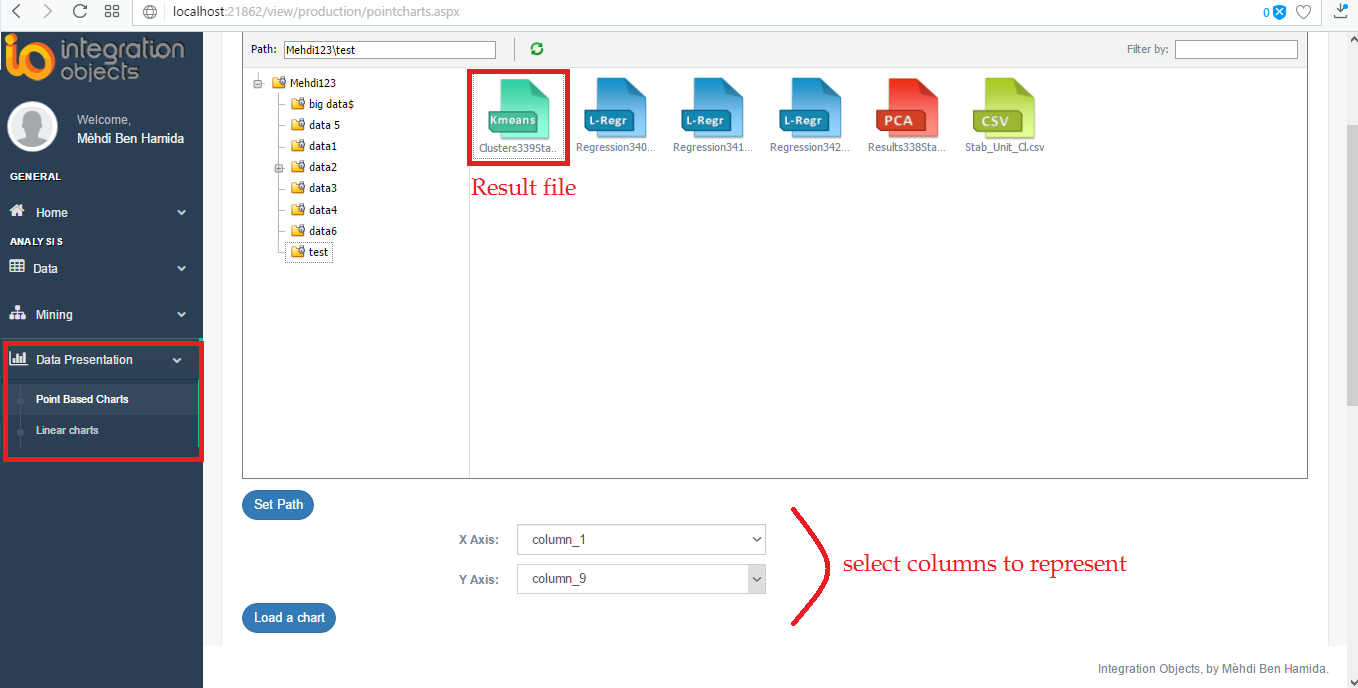
\includegraphics[width=17cm,height=10cm]{chapter5/kc1.png}
\end{center}
\caption{Set chart Parameters Page Capture}
\label{s3}
\end{figure} 


\item \textbf{Step 7:} Load chart\\


\begin{figure}[!ht]
\begin{center}
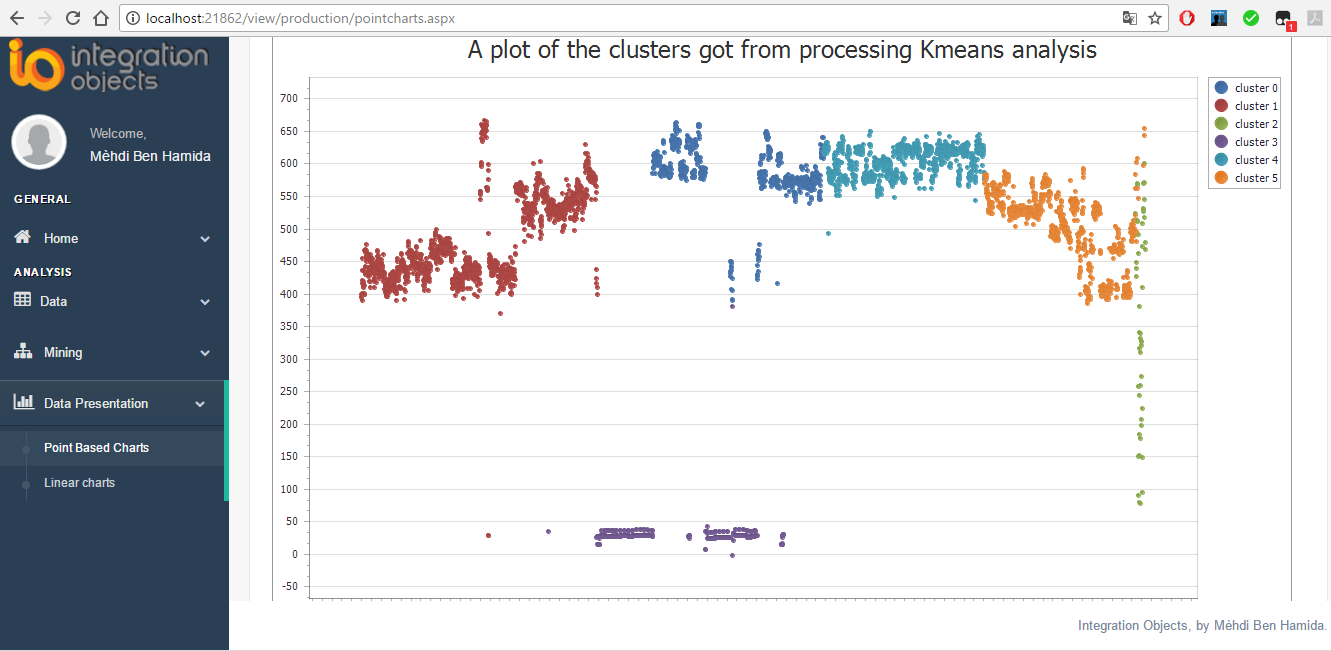
\includegraphics[width=17cm,height=10cm]{chapter5/kmeans.png}
\end{center}
\caption{Result Chart Capture}
\label{k}
\end{figure} 


\end{itemize}





\chapter{Principal Component Analysis}
\label{appendixpca}
The main problem of principal component analysis is represented by the equation represented in section \ref{sectionpca}:

\begin{equation*}
PX = (Px_{1} Px_{2} \ldots Px_{n})
=
\begin{pmatrix}
    p_{1}x_{1} & p_{1}x_{2}  & \dots  & p_{1}x_{n} \\
    p_{2}x_{1} & p_{2}x_{2}  & \dots  & p_{2}x_{n} \\
    \vdots & \vdots  & \ddots & \vdots \\
    p_{m}x_{1} & p_{m}x_{2}  & \dots  & p_{m}x_{n}
\end{pmatrix}
=
Y
\end{equation*}

Principal Components Analysis defines independence by considering the variance of the data in the original basis. It seeks to de-correlate the original data by finding the directions in which variance is maximised and the us these directions to define the new basis. Recall the definition for the variance of a random variable, $Z$ with mean, $\mu$.\\
\begin{equation*}
\sigma_{Z}^{2}=E[(Z-\mu )^{2}]
\end{equation*}

Suppose we have a vector of $n$ discrete measurement with mean $\mu_{r}$, if we subtract the mean from each of the measurement, then we obtain a translated set of measurement $r=(r_{1},r_{2},\ldots, r_{n},)$, that has zero mean. Thus, the variance of these measurement is given by the relation:\\
\begin{equation*}
\sigma_{r}^{2}=\frac{1}{n}rr^{T}
\end{equation*}

Suppose that we have a second vector of n measurement, $s = (s_{1}, s_{2}, \ldots ,s_{n})$, with zero mean, then we generalize this idea to obtain the covariance of $r$ and $s$. Covariance can be thought of as a measure of how much two variable change together. Variance is thus a special case of covariance, when the two variables are identical. It is in fact correct to divide through by a factor of $n-1$ rather than $n$.\\
\begin{equation*}
\sigma_{rs}^{2}=\dfrac{1}{n-1}rs^{T}
\end{equation*}

We can now generalize this idea to considering our $m \times n$ data matrix, $X$. Recall that m was the number of variables, and n the number of sample. We can therefore think of this matrix, $X$ in terms of $m$ row vectors, each of length n.\\
\begin{equation*}
X
=
\begin{pmatrix}
x_{1,1}&x_{1,2}&\cdots&x_{1,n}\\
x_{2,1}&x_{2,2}&\cdots&x_{2,n}\\
\vdots&\vdots&\ddots&\vdots\\
x_{m,1}&x_{m,1}&\cdots&x_{m,n}
\end{pmatrix} 
=
\begin{pmatrix}
X1\\
X2\\
\vdots\\
X_{m}
\end{pmatrix}
\in \mathbb{R}^{m\times n},\quad x_{i}^{T} \in \mathbb{R}^{n}
\end{equation*}

Since we have a row vector for each variable, each of these vectors contains all the samples for one particular variable. So for example, $x_{i}$ is a vector of the $n$ samples for the $i^{th}$ variable. It therefore makes sense to consider the following matrix product.\\
\begin{equation*}
C_{X}=\dfrac{1}{n-1}XX^{T}=\dfrac{1}{n-1}\begin{pmatrix}
X_{1}X_{1}^{T}&X_{1}X_{2}^{T}&\cdots &X_{1}X_{m}^{T}\\
X_{2}X_{1}^{T}&X_{2}X_{2}^{T}&\cdots &X_{2}X_{m}^{T}\\
\vdots &\vdots &\ddots &\vdots \\
X_{m}X_{1}^{T}&X_{m}X_{2}^{T}&\cdots &X_{m}X_{m}^{T}
\end{pmatrix}
\in \mathbb{R}^{m\times m}
\end{equation*}

If we look closely at the entries of this matrix, we see that we have computed all the possible covariance pairs between the $m$ variables. Indeed, on the diagonal entries, we have the variances and on the off-diagonal entries, we have the covariances. This matrix is therefore known as the Covariance Matrix.\\

Now let us return to the original problem, that of linearly transforming the original data matrix using the relation $Y=PX$, for some matrix, $P$. We need to decide upon some features that we would like the transformed matrix, $Y$ to exhibit and somehow relate this to the feature of the corresponding covarience matrix $C_{Y}$.\\

Covariance can be considered to be a mesure of how well correlated two variables are. The PCA method makes the fundamental assumption that the variables in the transformed matrix $C_{Y}$, should be as close to zero as possible (covariance matrices are always positive definite or positive semi-definite). Conversely, large variance values interest us, since they correspond to interesting dynamics in the system (small variances may well be noises). we therefore have the following requirements for constructing the covariance matrix, $C_{Y}$
\begin{itemize}
\item Maximise the signal, measured by variance (maximise the diagonal entries)
\item Minimise the covariance between variables (minimise the off-diagonal entries)\\
\end{itemize}

We thus come to the conclusion that since the minimum possible covariance is zero, we are seeking a diagonal matrix, $C_Y$. If we can choose the transformation matrix, $P$ in such a way that $C_Y$ is diagonal, then we will have achieved our objective.\\

We now make the assumption that the vectors in the new basis, $p_{1}, p_{2},\ldots , p_{m}$ are orthogonal (in fact, we additionally assume that they are orthonormal). Far from being restrictive, this assumption enables us to proceed by using the tools of linear algebra to find a solution to the problem. Consider the formula for the covariance matrix, $C_Y$ and our interpretation of $Y$ in terms of $X$ and $P$.\\
\begin{equation*}
\begin{multlined}
C_{Y} = \dfrac{1}{n-1} YY^{T} = \dfrac{1}{n-1} (PX)(PX)^T = \dfrac{1}{n-1} (PX)(X^{T}P^{T}) = \frac{1}{n-1} P(XX^{T})P^{T} \\
\quad \textrm{i.e} \quad C_{Y} = \dfrac{1}{n-1} PSP^{T} \quad \textrm{where} \quad  S = XX^{T}
\end{multlined}
\end{equation*}

Note that $S$ is an $ m \times n$ symmetric matrix, since $(XX^{T})^T = (X^T)^T(X)^{T}=XX^{T}$. We now invoke the well known theorem for linear algebra that every square symmetric matrix is orthogonally  (orthonormally) diagonalisable. That is, we can write:\\

\begin{equation*}
S=EDE^{T}
\end{equation*} 

Where E is an $m \times m$ orthonormal matrix whose columns are the orthonormal eigenvectors of $S$, and $D$ is the number of orthonormal eigenvectors that it has. if $B$ turns out to be rank-deficient so that $r$ is less than the size, $m$, of the matrix, then we simply need to generate $m-r$ orthonormal vectors to fill the remaining columns of $S$.\\
 
It is at this point that we make a choice for the transformation matrix, $P$. By choosing the rows of $P$ to be the eigenvectors of $S$, we ensure that $P=E^{T}$ and vice versa. Thus, substituting this into our derived expression for the covariance matrix, $C_Y$ gives:\\
\begin{equation*}
C_{Y} = \dfrac{1}{n-1}PSP^{T}=\dfrac{1}{n-1}E^{T}(EDE^{T})E
\end{equation*}

Now, since $E$ is an orthonormal matrix, we have $E^{T}E=I$ is the $m \times m$ identity matrix. Hence, for this special choice of $P$, we have:\\
\begin{equation*}
C_{Y}=\dfrac{1}{n-1}D
\end{equation*} 

A last point to note is that with this method, we automatically gain information about the relative importance of each principal component from the variances. The largest variance corresponds to the first principal component, the second largest to the second principal component, and so on. This therefore gives us a method for organising the data in the diagonalisation stage. Once we have obtained the eigenvalues and eigenvectors of $S = XX^{T}$, we sort the eigenvalues in descending order and place them in this order on the diagonal of $D$. We then construct the orthonormal matrix, $E$ by placing the associated eigenvectors in the same order to form the columns of $E$ (i.e. place the eigenvector that corresponds to the largest eigenvalue in the first column, the eigenvector corresponding to the second largest eigenvalue in the second column etc.).\\

We have therefore achieved our objective of diagonalising the covariance matrix of the
transformed data. The principal components (the rows of $P$) are the eigenvectors of the covariance matrix, $XX^{T}$, and the rows are in order of importance, telling us how principal each principal component is.

\end{appendix}
%\bibliography{./bibliographie.bib}
%voir wiki pour plus d'information sur la syntaxe des entrées d'une bibliographie

\end{document}